%-----------------------------------------------------------------------------------------
% Autor dieser Vorlage:
% Stefan Macke (http://fachinformatiker-anwendungsentwicklung.net)
% Permalink zur Vorlage: http://fiae.link/LaTeXVorlageFIAE
%
% Sämtliche verwendeten Abbildungen, Tabellen und Listings stammen von Dirk Grashorn.
%
% Lizenz: Creative Commons 4.0 Namensnennung - Weitergabe unter gleichen Bedingungen
% -----------------------------------------------------------------------------------------

\documentclass[
	ngerman,
	toc=listof, % Abbildungsverzeichnis sowie Tabellenverzeichnis in das Inhaltsverzeichnis aufnehmen
	toc=bibliography, % Literaturverzeichnis in das Inhaltsverzeichnis aufnehmen
	footnotes=multiple, % Trennen von direkt aufeinander folgenden Fußnoten
	parskip=half, % vertikalen Abstand zwischen Absätzen verwenden anstatt horizontale Einrückung von Folgeabsätzen
	numbers=noendperiod % Den letzten Punkt nach einer Nummerierung entfernen (nach DIN 5008)
]{scrartcl}
\pdfminorversion=5 % erlaubt das Einfügen von pdf-Dateien bis Version 1.7, ohne eine Fehlermeldung zu werfen (keine Garantie für fehlerfreies Einbetten!)
\usepackage[utf8]{inputenc} % muss als erstes eingebunden werden, da Meta/Packages ggfs. Sonderzeichen enthalten

% !TEX root = Projektdokumentation.tex

% Hinweis: der Titel muss zum Inhalt des Projekts passen und den zentralen Inhalt des Projekts deutlich herausstellen

\newcommand{\IHKlogo}{logo_handelskammer.png}
\newcommand{\titelOne}{Automatisierte Accounterstellung}
\newcommand{\titelTwo}{via AMQP-Messaging-System}
\newcommand{\untertitelOne}{mit Konsolidierung der Datenquellen}
\newcommand{\untertitelTwo}{(Übergabeprotokoll und Angebotssystem)}
\newcommand{\kompletterTitel}{\titelOne{}\\\titelTwo{}\\\untertitelOne{}\\\untertitelTwo{}}

\newcommand{\amqp}{amqp.png}
\newcommand{\netzplan}{netzplan.png}

\newcommand{\autorName}{Andreas Biller}

\newcommand{\betriebLogo}{logo_doctena.png}
\newcommand{\betriebLogoLower}{logo_doctena_lower.png}
\newcommand{\betriebName}{Doctena Germany GmbH}

\newcommand{\betriebAnschrift}{Urbanstr. 116}
\newcommand{\betriebOrt}{10967 Berlin}

\newcommand{\ausbildungsberuf}{Fachinformatiker für Anwendungsentwicklung}
\newcommand{\betreff}{Dokumentation zur betrieblichen Projektarbeit}

\newcommand{\abgabeOrt}{Berlin}
\newcommand{\abgabeTermin}{24.05.2018} % Metadaten zu diesem Dokument (Autor usw.)
% !TEX root = ../Projektdokumentation.tex

% Anpassung an Landessprache ---------------------------------------------------
\usepackage{babel}

% Umlaute ----------------------------------------------------------------------
%   Umlaute/Sonderzeichen wie äüöß direkt im Quelltext verwenden (CodePage).
%   Erlaubt automatische Trennung von Worten mit Umlauten.
% ------------------------------------------------------------------------------
\usepackage[T1]{fontenc}
\usepackage{textcomp} % Euro-Zeichen etc.

% Schrift ----------------------------------------------------------------------
\usepackage{lmodern} % bessere Fonts
\usepackage{relsize} % Schriftgröße relativ festlegen

% Tabellen ---------------------------------------------------------------------
\PassOptionsToPackage{table}{xcolor}
\usepackage{tabularx}
% für lange Tabellen
\usepackage{longtable}
\usepackage{array}
\usepackage{ragged2e}
\usepackage{lscape}
\newcolumntype{w}[1]{>{\raggedleft\hspace{0pt}}p{#1}} % Spaltendefinition rechtsbündig mit definierter Breite

% Grafiken ---------------------------------------------------------------------
\usepackage[dvips,final]{graphicx} % Einbinden von JPG-Grafiken ermöglichen
\usepackage{graphics} % keepaspectratio
\usepackage{floatflt} % zum Umfließen von Bildern
\graphicspath{{Bilder/}} % hier liegen die Bilder des Dokuments

% Sonstiges --------------------------------------------------------------------
\usepackage[titles]{tocloft} % Inhaltsverzeichnis DIN 5008 gerecht einrücken
\usepackage{amsmath,amsfonts} % Befehle aus AMSTeX für mathematische Symbole
\usepackage{enumitem} % anpassbare Enumerates/Itemizes
\usepackage{xspace} % sorgt dafür, dass Leerzeichen hinter parameterlosen Makros nicht als Makroendezeichen interpretiert werden

\usepackage{makeidx} % für Index-Ausgabe mit \printindex
\usepackage[printonlyused]{acronym} % es werden nur benutzte Definitionen aufgelistet

% Einfache Definition der Zeilenabstände und Seitenränder etc.
\usepackage{setspace}
\usepackage{geometry}

% Symbolverzeichnis
\usepackage[intoc]{nomencl}
\let\abbrev\nomenclature
\renewcommand{\nomname}{Abkürzungsverzeichnis}
\setlength{\nomlabelwidth}{.25\hsize}
\renewcommand{\nomlabel}[1]{#1 \dotfill}
\setlength{\nomitemsep}{-\parsep}

\usepackage{varioref} % Elegantere Verweise. „auf der nächsten Seite“
\usepackage{url} % URL verlinken, lange URLs umbrechen etc.

\usepackage{chngcntr} % fortlaufendes Durchnummerieren der Fußnoten
% \usepackage[perpage]{footmisc} % Alternative: Nummerierung der Fußnoten auf jeder Seite neu

\usepackage{ifthen} % bei der Definition eigener Befehle benötigt
\usepackage{todonotes} % definiert u.a. die Befehle \todo und \listoftodos
\usepackage[square]{natbib} % wichtig für korrekte Zitierweise

% PDF-Optionen -----------------------------------------------------------------
\usepackage{pdfpages}
\pdfminorversion=5 % erlaubt das Einfügen von pdf-Dateien bis Version 1.7, ohne eine Fehlermeldung zu werfen (keine Garantie für fehlerfreies Einbetten!)
\usepackage[
    bookmarks,
    bookmarksnumbered,
    bookmarksopen=true,
    bookmarksopenlevel=1,
    colorlinks=true,
% diese Farbdefinitionen zeichnen Links im PDF farblich aus
    linkcolor=AOBlau, % einfache interne Verknüpfungen
    anchorcolor=AOBlau,% Ankertext
    citecolor=AOBlau, % Verweise auf Literaturverzeichniseinträge im Text
    filecolor=AOBlau, % Verknüpfungen, die lokale Dateien öffnen
    menucolor=AOBlau, % Acrobat-Menüpunkte
    urlcolor=AOBlau,
% diese Farbdefinitionen sollten für den Druck verwendet werden (alles schwarz)
    %linkcolor=black, % einfache interne Verknüpfungen
    %anchorcolor=black, % Ankertext
    %citecolor=black, % Verweise auf Literaturverzeichniseinträge im Text
    %filecolor=black, % Verknüpfungen, die lokale Dateien öffnen
    %menucolor=black, % Acrobat-Menüpunkte
    %urlcolor=black,
%
    %backref, % Quellen werden zurück auf ihre Zitate verlinkt
    pdftex,
    plainpages=false, % zur korrekten Erstellung der Bookmarks
    pdfpagelabels=true, % zur korrekten Erstellung der Bookmarks
    hypertexnames=false, % zur korrekten Erstellung der Bookmarks
    linktocpage % Seitenzahlen anstatt Text im Inhaltsverzeichnis verlinken
]{hyperref}
% Befehle, die Umlaute ausgeben, führen zu Fehlern, wenn sie hyperref als Optionen übergeben werden
\hypersetup{
    pdftitle={\titel -- \untertitel},
    pdfauthor={\autorNameOne -- \autorNameTwo},
    pdfcreator={\autorNameOne -- \autorNameTwo},
    pdfsubject={\titel -- \untertitel},
    pdfkeywords={\titel -- \untertitel},
}


% zum Einbinden von Programmcode -----------------------------------------------
\usepackage{listings}
\usepackage{xcolor}
\definecolor{hellgelb}{rgb}{1,1,0.9}
\definecolor{colKeys}{rgb}{0,0,1}
\definecolor{colIdentifier}{rgb}{0,0,0}
\definecolor{colComments}{rgb}{0,0.5,0}
\definecolor{colString}{rgb}{1,0,0}
\lstset{
    float=hbp,
	basicstyle=\footnotesize,
    identifierstyle=\color{colIdentifier},
    keywordstyle=\color{colKeys},
    stringstyle=\color{colString},
    commentstyle=\color{colComments},
    backgroundcolor=\color{hellgelb},
    columns=flexible,
    tabsize=2,
    frame=single,
    extendedchars=true,
    showspaces=false,
    showstringspaces=false,
    numbers=left,
    numberstyle=\tiny,
    breaklines=true,
    breakautoindent=true,
	captionpos=b,
}
\lstdefinelanguage{cs}{
	sensitive=false,
	morecomment=[l]{//},
	morecomment=[s]{/*}{*/},
	morestring=[b]",
	morekeywords={
		abstract,event,new,struct,as,explicit,null,switch
		base,extern,object,this,bool,false,operator,throw,
		break,finally,out,true,byte,fixed,override,try,
		case,float,params,typeof,catch,for,private,uint,
		char,foreach,protected,ulong,checked,goto,public,unchecked,
		class,if,readonly,unsafe,const,implicit,ref,ushort,
		continue,in,return,using,decimal,int,sbyte,virtual,
		default,interface,sealed,volatile,delegate,internal,short,void,
		do,is,sizeof,while,double,lock,stackalloc,
		else,long,static,enum,namespace,string},
}
\lstdefinelanguage{natural}{
	sensitive=false,
	morecomment=[l]{/*},
	morestring=[b]",
	morestring=[b]',
	alsodigit={-,*},
	morekeywords={
		DEFINE,DATA,LOCAL,END-DEFINE,WRITE,CALLNAT,PARAMETER,USING,
		IF,NOT,END-IF,ON,*ERROR-NR,ERROR,END-ERROR,ESCAPE,ROUTINE,
		PERFORM,SUBROUTINE,END-SUBROUTINE,CONST,END-FOR,END,FOR,RESIZE,
		ARRAY,TO,BY,VALUE,RESET,COMPRESS,INTO,EQ},
}
\lstdefinelanguage{php}{
	sensitive=false,
	morecomment=[l]{/*},
	morestring=[b]",
	morestring=[b]',
	alsodigit={-,*},
	morekeywords={
		abstract,and,array,as,break,case,catch,cfunction,class,clone,const,
		continue,declare,default,do,else,elseif,enddeclare,endfor,endforeach,
		endif,endswitch,endwhile,extends,final,for,foreach,function,global,
		goto,if,implements,interface,instanceof,namespace,new,old_function,or,
		private,protected,public,static,switch,throw,try,use,var,while,xor
		die,echo,empty,exit,eval,include,include_once,isset,list,require,
		require_once,return,print,unset},
}

% fix errors
\usepackage{scrhack}
 % verwendete Packages
% !TEX root = ../Projektdokumentation.tex

% Seitenränder -----------------------------------------------------------------
\setlength{\topskip}{\ht\strutbox} % behebt Warnung von geometry
\geometry{a4paper,left=20mm,right=20mm,top=25mm,bottom=35mm}

\usepackage[
	automark, % Kapitelangaben in Kopfzeile automatisch erstellen
	headsepline, % Trennlinie unter Kopfzeile
	ilines % Trennlinie linksbündig ausrichten
]{scrpage2}

% Kopf- und Fußzeilen ----------------------------------------------------------
\pagestyle{scrheadings}
% chapterpagestyle gibt es nicht in scrartcl
%\renewcommand{\chapterpagestyle}{scrheadings}
\clearscrheadfoot

% Kopfzeile
\renewcommand{\headfont}{\normalfont} % Schriftform der Kopfzeile
\ihead{\large{\textsc{\titel}}\\ \small{\untertitel} \\[2ex] \textit{\headmark}}
\chead{}
\ohead{\includegraphics[scale=0.4]{\betriebLogo}}
\setlength{\headheight}{15mm} % Höhe der Kopfzeile
%\setheadwidth[0pt]{textwithmarginpar} % Kopfzeile über den Text hinaus verbreitern (falls Logo den Text überdeckt)

% Fußzeile
\ifoot{\autorName}
\cfoot{}
\ofoot{\pagemark}

% Überschriften nach DIN 5008 in einer Fluchtlinie
% ------------------------------------------------------------------------------

% Abstand zwischen Nummerierung und Überschrift definieren
% > Schön wäre hier die dynamische Berechnung des Abstandes in Abhängigkeit
% > der Verschachtelungstiefe des Inhaltsverzeichnisses
\newcommand{\headingSpace}{1.5cm}

% Abschnittsüberschriften im selben Stil wie beim Inhaltsverzeichnis einrücken
\renewcommand*{\othersectionlevelsformat}[3]{
  \makebox[\headingSpace][l]{#3\autodot}
}

% Für die Einrückung wird das Paket tocloft benötigt
%\cftsetindents{chapter}{0.0cm}{\headingSpace}
\cftsetindents{section}{0.0cm}{\headingSpace}
\cftsetindents{subsection}{0.0cm}{\headingSpace}
\cftsetindents{subsubsection}{0.0cm}{\headingSpace}
\cftsetindents{figure}{0.0cm}{\headingSpace}
\cftsetindents{table}{0.0cm}{\headingSpace}


% Allgemeines
% ------------------------------------------------------------------------------

\onehalfspacing % Zeilenabstand 1,5 Zeilen
\frenchspacing % erzeugt ein wenig mehr Platz hinter einem Punkt

% Schusterjungen und Hurenkinder vermeiden
\clubpenalty = 10000
\widowpenalty = 10000
\displaywidowpenalty = 10000

% Quellcode-Ausgabe formatieren
\lstset{numbers=left, numberstyle=\tiny, numbersep=5pt, breaklines=true}
\lstset{emph={square}, emphstyle=\color{red}, emph={[2]root,base}, emphstyle={[2]\color{blue}}}

\counterwithout{footnote}{section} % Fußnoten fortlaufend durchnummerieren
\setcounter{tocdepth}{\subsubsectionlevel} % im Inhaltsverzeichnis werden die Kapitel bis zum Level der subsubsection übernommen
\setcounter{secnumdepth}{\subsubsectionlevel} % Kapitel bis zum Level der subsubsection werden nummeriert

% Aufzählungen anpassen
\renewcommand{\labelenumi}{\arabic{enumi}.}
\renewcommand{\labelenumii}{\arabic{enumi}.\arabic{enumii}.}
\renewcommand{\labelenumiii}{\arabic{enumi}.\arabic{enumii}.\arabic{enumiii}}

% Tabellenfärbung:
\definecolor{heading}{rgb}{0.64,0.78,0.86}
\definecolor{odd}{rgb}{0.9,0.9,0.9}
 % Definitionen zum Aussehen der Seiten
% !TEX root = ../Projektdokumentation.tex

% Abkürzungen, ggfs. mit korrektem Leerraum
\newcommand{\bs}{$\backslash$\xspace}
\newcommand{\bspw}{bspw.\xspace}
\newcommand{\bzw}{bzw.\xspace}
\newcommand{\ca}{ca.\xspace}
\newcommand{\dahe}{\mbox{d.\,h.}\xspace}
\newcommand{\etc}{etc.\xspace}
\newcommand{\eur}[1]{\mbox{#1\,\texteuro}\xspace}
\newcommand{\evtl}{evtl.\xspace}
\newcommand{\ggfs}{ggfs.\xspace}
\newcommand{\Ggfs}{Ggfs.\xspace}
\newcommand{\gqq}[1]{\glqq{}#1\grqq{}}
\newcommand{\inkl}{inkl.\xspace}
\newcommand{\insb}{insb.\xspace}
\newcommand{\ua}{\mbox{u.\,a.}\xspace}
\newcommand{\usw}{usw.\xspace}
\newcommand{\Vgl}{Vgl.\xspace}
\newcommand{\zB}{\mbox{z.\,B.}\xspace}

% Befehle für häufig anfallende Aufgaben
\newcommand{\Abbildung}[1]{\autoref{fig:#1}}
\newcommand{\Anhang}[1]{\appendixname{}~\ref{#1}: \nameref{#1} \vpageref{#1}}
\newcommand{\includegraphicsKeepAspectRatio}[2]{\includegraphics[width=#2\textwidth,height=#2\textheight,keepaspectratio]{#1}}
\newcommand{\Zitat}[2][\empty]{\ifthenelse{\equal{#1}{\empty}}{\citep{#2}}{\citep[#1]{#2}}}
\newcommand{\Autor}[1]{\textsc{#1}} % zum Ausgeben von Autoren
\newcommand{\itemd}[2]{\item{\textbf{#1}}\\{#2}} % erzeugt ein Listenelement mit fetter Überschrift

% fügt Tabellen aus einer TEX-Datei ein
\newcommand{\tabelle}[3] % Parameter: caption, label, file
{\begin{table}[htbp]
\centering
\singlespacing
\input{Tabellen/#3}
\caption{#1}
\label{#2}
\end{table}}

\newcommand{\tabelleAnhang}[1] % Parameter: file
{\begin{center}
\singlespacing
\input{Tabellen/#1}
\end{center}}

% einfaches Wechseln der Schrift, z.B.: \changefont{cmss}{sbc}{n}
\newcommand{\changefont}[3]{\fontfamily{#1} \fontseries{#2} \fontshape{#3} \selectfont}

% Verwendung analog zu \includegraphics
\newlength{\myx} % Variable zum Speichern der Bildbreite
\newlength{\myy} % Variable zum Speichern der Bildhöhe
\newcommand\includegraphicstotab[2][\relax]{%
% Abspeichern der Bildabmessungen
\settowidth{\myx}{\includegraphics[{#1}]{#2}}%
\settoheight{\myy}{\includegraphics[{#1}]{#2}}%
% das eigentliche Einfügen
\parbox[c][1.1\myy][c]{\myx}{%
\includegraphics[{#1}]{#2}}%
}

\definecolor{AOBlau}{rgb}{0, 0.28, 0.56}

% verschiedene Befehle um Wörter semantisch auszuzeichnen ----------------------
\newcommand{\Index}[2][\empty]{\ifthenelse{\equal{#1}{\empty}}{\index{#2}#2}{\index{#1}#2}}
\newcommand{\Fachbegriff}[2][\empty]{\ifthenelse{\equal{#1}{\empty}}{\textit{\Index{#2}}}{\textit{\Index[#1]{#2}}}}
\newcommand{\NeuerBegriff}[2][\empty]{\ifthenelse{\equal{#1}{\empty}}{\textbf{\Index{#2}}}{\textbf{\Index[#1]{#2}}}}

\newcommand{\Ausgabe}[1]{\texttt{#1}}
\newcommand{\Eingabe}[1]{\texttt{#1}}
\newcommand{\Code}[1]{\texttt{#1}}
\newcommand{\Datei}[1]{\texttt{#1}}

\newcommand{\Assembly}[1]{\textsf{#1}}
\newcommand{\Klasse}[1]{\textsf{#1}}
\newcommand{\Methode}[1]{\textsf{#1}}
\newcommand{\Attribut}[1]{\textsf{#1}}

\newcommand{\Datentyp}[1]{\textsf{#1}}
\newcommand{\XMLElement}[1]{\textsf{#1}}
\newcommand{\Webservice}[1]{\textsf{#1}}

\newcommand{\Refactoring}[1]{\Fachbegriff{#1}}
\newcommand{\CodeSmell}[1]{\Fachbegriff{#1}}
\newcommand{\Metrik}[1]{\Fachbegriff{#1}}
\newcommand{\DesignPattern}[1]{\Fachbegriff{#1}}
 % eigene allgemeine Befehle, die z.B. die Arbeit mit LaTeX erleichtern
% !TEX root = ../Projektdokumentation.tex

% Abkürzungen, ggfs. mit korrektem Leerraum
\newcommand{\bs}{$\backslash$\xspace}
\newcommand{\bspw}{bspw.\xspace}
\newcommand{\bzw}{bzw.\xspace}
\newcommand{\ca}{ca.\xspace}
\newcommand{\dahe}{\mbox{d.\,h.}\xspace}
\newcommand{\etc}{etc.\xspace}
\newcommand{\eur}[1]{\mbox{#1\,\texteuro}\xspace}
\newcommand{\evtl}{evtl.\xspace}
\newcommand{\ggfs}{ggfs.\xspace}
\newcommand{\Ggfs}{Ggfs.\xspace}
\newcommand{\gqq}[1]{\glqq{}#1\grqq{}}
\newcommand{\inkl}{inkl.\xspace}
\newcommand{\insb}{insb.\xspace}
\newcommand{\ua}{\mbox{u.\,a.}\xspace}
\newcommand{\usw}{usw.\xspace}
\newcommand{\Vgl}{Vgl.\xspace}
\newcommand{\zB}{\mbox{z.\,B.}\xspace}

% Befehle für häufig anfallende Aufgaben
\newcommand{\Abbildung}[1]{\autoref{fig:#1}}
\newcommand{\Anhang}[1]{\appendixname{}~\ref{#1}: \nameref{#1} \vpageref{#1}}
\newcommand{\includegraphicsKeepAspectRatio}[2]{\includegraphics[width=#2\textwidth,height=#2\textheight,keepaspectratio]{#1}}
\newcommand{\Zitat}[2][\empty]{\ifthenelse{\equal{#1}{\empty}}{\citep{#2}}{\citep[#1]{#2}}}
\newcommand{\Autor}[1]{\textsc{#1}} % zum Ausgeben von Autoren
\newcommand{\itemd}[2]{\item{\textbf{#1}}\\{#2}} % erzeugt ein Listenelement mit fetter Überschrift

% fügt Tabellen aus einer TEX-Datei ein
\newcommand{\tabelle}[3] % Parameter: caption, label, file
{\begin{table}[htbp]
\centering
\singlespacing
\input{Tabellen/#3}
\caption{#1}
\label{#2}
\end{table}}

\newcommand{\tabelleAnhang}[1] % Parameter: file
{\begin{center}
\singlespacing
\input{Tabellen/#1}
\end{center}}

% einfaches Wechseln der Schrift, z.B.: \changefont{cmss}{sbc}{n}
\newcommand{\changefont}[3]{\fontfamily{#1} \fontseries{#2} \fontshape{#3} \selectfont}

% Verwendung analog zu \includegraphics
\newlength{\myx} % Variable zum Speichern der Bildbreite
\newlength{\myy} % Variable zum Speichern der Bildhöhe
\newcommand\includegraphicstotab[2][\relax]{%
% Abspeichern der Bildabmessungen
\settowidth{\myx}{\includegraphics[{#1}]{#2}}%
\settoheight{\myy}{\includegraphics[{#1}]{#2}}%
% das eigentliche Einfügen
\parbox[c][1.1\myy][c]{\myx}{%
\includegraphics[{#1}]{#2}}%
}

\definecolor{AOBlau}{rgb}{0, 0.28, 0.56}

% verschiedene Befehle um Wörter semantisch auszuzeichnen ----------------------
\newcommand{\Index}[2][\empty]{\ifthenelse{\equal{#1}{\empty}}{\index{#2}#2}{\index{#1}#2}}
\newcommand{\Fachbegriff}[2][\empty]{\ifthenelse{\equal{#1}{\empty}}{\textit{\Index{#2}}}{\textit{\Index[#1]{#2}}}}
\newcommand{\NeuerBegriff}[2][\empty]{\ifthenelse{\equal{#1}{\empty}}{\textbf{\Index{#2}}}{\textbf{\Index[#1]{#2}}}}

\newcommand{\Ausgabe}[1]{\texttt{#1}}
\newcommand{\Eingabe}[1]{\texttt{#1}}
\newcommand{\Code}[1]{\texttt{#1}}
\newcommand{\Datei}[1]{\texttt{#1}}

\newcommand{\Assembly}[1]{\textsf{#1}}
\newcommand{\Klasse}[1]{\textsf{#1}}
\newcommand{\Methode}[1]{\textsf{#1}}
\newcommand{\Attribut}[1]{\textsf{#1}}

\newcommand{\Datentyp}[1]{\textsf{#1}}
\newcommand{\XMLElement}[1]{\textsf{#1}}
\newcommand{\Webservice}[1]{\textsf{#1}}

\newcommand{\Refactoring}[1]{\Fachbegriff{#1}}
\newcommand{\CodeSmell}[1]{\Fachbegriff{#1}}
\newcommand{\Metrik}[1]{\Fachbegriff{#1}}
\newcommand{\DesignPattern}[1]{\Fachbegriff{#1}}
 % eigene projektspezifische Befehle, z.B. Abkürzungen usw.



\begin{document}

% \phantomsection
% \thispagestyle{empty}
% \pdfbookmark[1]{Eidesstattliche Erklärung}{ihkdeckblatt}
% \includegraphicsKeepAspectRatio{DeckblattIHK}{1}
% \cleardoublepage

\phantomsection
\thispagestyle{plain}
\pdfbookmark[1]{Deckblatt}{deckblatt}
% !TEX root = Projektdokumentation.tex
\begin{titlepage}

\begin{center}
\includegraphics[scale=0.2]{\IHKlogo}\\[0.5ex]
\Large{\ausbildungsberuf}\\
\LARGE{\betreff}\\
\huge{\textbf{\titelOne\\\titelTwo}}\\[0.5ex]
\Large{\textbf{\untertitelOne}}\\
\Large{\textbf{\untertitelTwo}}\\[1.5ex]

\normalsize
\textbf{Auszubildender:} \autorName\\[2.5ex]

\begin{figure}[htb]
    \centering
    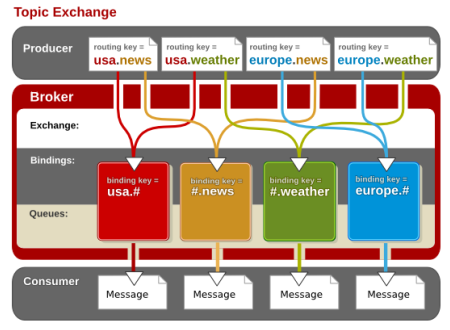
\includegraphics[scale=0.85]{\amqp}\\[1ex]
    \caption{Versand von Nachrichten mittels \ac{AMQP}}
    \label{fig:DMZ_Korea}
\end{figure}

\textbf{Abgabetermin:} \abgabeOrt{}, den \abgabeTermin\\[3ex]

\includegraphics[scale=0.45]{\betriebLogo}\\
\betriebName{}\\
\betriebAnschrift{}, \betriebOrt\\[2.5ex]
\end{center}

\small
\noindent
Dieses Werk einschließlich seiner Teile ist \textbf{urheberrechtlich geschützt}.
Jede Verwertung außerhalb der engen Grenzen des Urheberrechtsgesetzes ist ohne Zustimmung des Autors unzulässig und strafbar.
Das gilt insbesondere für Vervielfältigungen, Übersetzungen, Mikroverfilmungen sowie die Einspeicherung und Verarbeitung in elektronischen Systemen.

\end{titlepage}
\cleardoublepage

% Preface --------------------------------------------------------------------
\phantomsection
\pagenumbering{Roman}
\pdfbookmark[1]{Inhaltsverzeichnis}{inhalt}
\tableofcontents
\cleardoublepage

\phantomsection
\listoffigures
\cleardoublepage

\phantomsection
\listoftables
\cleardoublepage

\phantomsection
\lstlistoflistings
\cleardoublepage

\newcommand{\abkvz}{Abkürzungsverzeichnis}
\renewcommand{\nomname}{\abkvz}
\section*{\abkvz}
\markboth{\abkvz}{\abkvz}
\addcontentsline{toc}{section}{\abkvz}
% !TEX root = Projektdokumentation.tex

% Es werden nur die Abkürzungen aufgelistet, die mit \ac definiert und auch benutzt wurden. 
%
% \acro{VERSIS}{Versicherungsinformationssystem\acroextra{ (Bestandsführungssystem)}}
% Ergibt in der Liste: VERSIS Versicherungsinformationssystem (Bestandsführungssystem)
% Im Text aber: \ac{VERSIS} -> Versicherungsinformationssystem (VERSIS)

% Hinweis: allgemein bekannte Abkürzungen wie z.B. bzw. u.a. müssen nicht ins Abkürzungsverzeichnis aufgenommen werden
% Hinweis: allgemein bekannte IT-Begriffe wie Datenbank oder Programmiersprache müssen nicht erläutert werden,
%          aber ggfs. Fachbegriffe aus der Domäne des Prüflings (z.B. Versicherung)

% Die Option (in den eckigen Klammern) enthält das längste Label oder
% einen Platzhalter der die Breite der linken Spalte bestimmt.
\begin{acronym}[WWWWWW]
    \acro{AMQP}{Advanced Message Queuing Protocol}
    \acro{BASH}{Bourne Again Shell}
    \acro{CAS}{Column Access Strobe}
    \acro{CL}{\ac{CAS} latency}
    \acro{CLI}{Command Line Interface}
    \acro{DDR4}{Double Data Rate 4th-Generation}
    \acro{DHCP}{Dynamic Host Configuration Protocol}
    \acro{DIMM}{Dual In-line Memory Module}
	\acro{DMZ}{Demilitarisierte Zone}
    \acro{DNS}{Domain Name Server}
    \acro{FA}{Fachinformatik für Anwendungsentwicklung}
    \acro{FTP}{File Transfer Protokoll}
    \acro{GB}{Giga Byte}
    \acro{GHz}{Giga Hertz}
    \acro{GUI}{Graphical User Interface}
    \acro{HTML}{Hypertext Markup Language}
    \acro{ICMP}{Internet Control Message Protocol}
    \acro{ID}{Identification}
	\acro{IHK}{Industrie- und Handelskammer}
    \acro{IP}{Internet Protokoll}
    \acro{IT}{Informationstechnik}
	\acro{ITS}{Informationstechnische Systeme}
    \acro{LAN}{Local Area Network}
    \acro{LPI}{Linux Professional Institute}
    \acro{MB}{Mega Byte}
    \acro{NAT}{Network Adress Translation}
    \acro{NTP}{Network Time Protocol}
    \acro{OSZIMT}{Oberstufenzentrum Informations- und Medizintechnik}
    \acro{PC}{Personal Computer}
	\acro{P/LZ}{Projekt/Linux-Zertifizierung}
    \acro{RAM}{Random Access Memory}
    \acro{SSD}{Solid State Drive}
    \acro{SSH}{Secure Shell}
    \acro{TCP}{Transmission Control Protocol}
    \acro{UDP}{User Datagram Protocol}
    \acro{VLAN}{Virtual \ac{LAN}}
    \acro{VM}{Virtual Machine}
\end{acronym}

\clearpage

% Inhalt ---------------------------------------------------------------------
\pagenumbering{arabic}
% !TEX root = Projektdokumentation.tex
% !TEX root = ../Projektdokumentation.tex
\section{Einleitung}
\label{sec:Einleitung}
% TODO: Zitat finden, in dem es um den Wert der eigenständigen Projektarbeit geht, und dann hier einfügen.
\begin{quote}
\textit{Pläne sind nichts, Planung ist alles.}\\
Dwight D. Eisenhower, ehemaliger US-Präsident
\end{quote}
\begin{quote}
\textit{Kein Plan überlebt die erste Feindberührung.}\\
Helmuth von Moltke, preußischer Generalfeldmarschall
\end{quote}

\subsection{Projektumfeld} 
\label{sec:Projektumfeld}
% Kurze Vorstellung des Ausbildungsbetriebs (Geschäftsfeld, Mitarbeiterzahl \usw)
Das Projekt wird als Teil der Abschlussprüfung im Rahmen meiner Ausbildung zum Fachinformatiker für Anwendungsentwicklung bei der Doctena Germany GmbH umgesetzt. Doctena ist ein internationales Unternehmen mit Hauptsitz in Luxemburg und Niederlassungen in 5 weiteren europäischen Ländern. Doctena bietet Patienten eine internationale Plattform zur Online-Terminbuchung an. "2013 (\dots) wurde die Plattform Doctena in Luxemburg ins Leben gerufen. (\dots) Aufgrund des anhaltenden Erfolges und des schnellen Wachstums des Projekts dehnte das Unternehmen seine Aktivitäten auf Belgien, die Niederlande, [Österreich,] die Schweiz und Deutschland aus. Seit 2016 hat sich Doctena mit sechs Wettbewerbern zusammengeschlossen: DocBook (BE), Doxter (DE), Terminland (DE), Sanmax (BE), Mednanny (AT) und Bookmydoc (LU). Doctena ist heute die führende medizinische Buchungsplattform in Europa."\footnote{Über Doctena - Unsere Firma - Eine Erfolgsgeschichte, \cite{wwwDoctenaComOne}} Doctena beschäftigt momentan um die 80 Mitarbeiter, ca. 30 davon hier in Berlin. Hauptprodukt neben der Terminbuchungs-Plattform für Patienten ist die cloudbasierte Terminverwaltungs-Lösung Doctena Pro für Ärzte und Praxen. "Doctena hat das Ziel, den Zugriff von Patienten auf verfügbare Termine von Ärzten und Praktikern zu vereinfachen. Patienten können mit Hilfe der Onlineplattform oder der Handy-App verfügbare Termine sehen und buchen. (\dots) Die Lösung ist mit vielen medizinischen Buchungssoftwares kompatibel und kann deshalb leicht in die Struktur von Ärzten und ihren Praxen integriert werden."\footnote{Über Doctena - Der Doctena Update Catalog, \cite{wwwDoctenaComTwo}} So können Ärzte praxisintern ihre Verfügbarkeiten managen und gleichzeitig freie Termine über die Plattform oder über die eigene Internetseite anbieten.
% Wer ist Auftraggeber/Kunde des Projekts?
Eigentlicher Kunde des Projektes sind die Abteilungen Verkauf und Onboarding der Doctena Germany GmbH. Die Abnahme des Projekts erfolgt durch den \ac{CTO} der Doctena Germany GmbH, André Rauschenbach.

\subsection{Projektziel} 
\label{sec:Projektziel}
% Worum geht es eigentlich?
% Was soll erreicht werden?
Ziel des Projektes ist die Erweiterung des zur Angebots- und Vertragserstellung benutzten Angebotssystemes. Den Onboarding-Managern soll damit ermöglicht werden, nach Annahme des Angebotes durch den Kunden, in unserem System die automatische Accounterstellung auf dem luxemburger System Doctena Pro über den bestehenden \ac{AMQP} Message-Bus auszulösen. Zusätzlich soll die Maske des Angebotsformulars um Eingabefelder für das in Folge zu erstellende Übergabeprotokoll erweitert und so eine Konsolidierung der bisher für den Onboarding-Prozess verwendeten Datenquellen erreicht werden.

\subsection{Projektbegründung} 
\label{sec:Projektbegruendung}
% Warum ist das Projekt sinnvoll (\zB Kosten- oder Zeitersparnis, weniger Fehler)?
Mit diesem Projekt soll die bisherige manuelle Erstellung der neuen Kunden-Accounts durch die Onboarding-Manager automatisiert werden, was zu einer Zeit- und somit auch Kostenreduzierung im Onboarding-Prozess führt. Gleichzeitig sollen mögliche Fehlerquellen bei der im bisherigen Prozess hierzu verwendeten doppelten Datenhaltung eliminiert werden.
% Was ist die Motivation hinter dem Projekt?
Hauptmotivation hinter dem Projekt ist somit die Prozessoptimierung bei der bisherigen Accounterstellung. Neben dem reinen Arbeitsaufwand sollen hiermit auch Fehler reduziert werden, die durchdie vielen repetitive Aufgaben beim Onboarding und anspruchslose Copy-und-Paste-Tätigkeiten leicht entstehen können.

\subsection{Projektschnittstellen} 
\label{sec:Projektschnittstellen}
% Mit welchen anderen Systemen interagiert die Anwendung (technische Schnittstellen)?
Das Angebotssystem im Backend des deutschen Systems Doctena Standard wurde mit Ruby on Rails erstellt. Es besteht eine Verbindung zu einer nicht-relationalen MongoDB Datenbank über einen in Rails eingebundenen Data-Connector, den MongoDB Driver. Die browserbasierte Eingabemaske des Views kann so unabhängig vom verwendeten Betriebsystem benutzt werden.
Die externe Kommunikation zwischen den Objekten in Rails bei Doctena Standard und den Objekten im Zielsystem Doctena Pro, mit denen der neue Benutzeraccount nach Vertragserstellung angelegt werden soll, erfolgt über einen \ac{AMQP} Message-Bus mit RabbitMQ. Dieser wird bereits zur Synchronisation der Verfügbarkeiten der Ärzte aus den verschiedenen Backend-Bereichen der angeschlossenen Systeme mit dem \ac{CPP} von Doctena benutzt. Die verwendete Datenstruktur zum Versand der Objekte ist  ßac{JSON}.
% Wer genehmigt das Projekt \bzw stellt Mittel zur Verfügung? 
Das Projekt wurde von Doctenas internationalem \ac{CIO}, Alain Fountain, in Absprache mit dem  \ac{CTO} von Doctena Germany, André Rauschenbach, genehmigt. Doctena stellt somit als Kunde im Rahmen der Projektarbeit und Ausbildung alle zur Umsetzung benötigten Mittel zur Verfügung.
% Wer sind die Benutzer der Anwendung?
Benutzer der Anwendung sind die Mitarbeiter von Doctena Germany in den Abteilungen Verkauf und Onboarding.
% Wem muss das Ergebnis präsentiert werden?
Diesen soll nach Abnahme durch den Auftraggeber, vertreten durch den \ac{CTO} von Doctena Germany, das fertige Produkt präsentiert werden. Zusätzlich soll für die Benutzer eine Benutzerdokumentation für die Accounterstellung im Firmeninternen Wiki erstellt werden.

\subsection{Projektabgrenzung} 
\label{sec:Projektabgrenzung}
Das Aktivieren von Features über den Bus ist Seitens Luxemburg noch nicht möglich. Deswegen wurde diese Funktionalität aus dem Projekt ausgeklammert. Sie wird erst zu einem späteren Zeitpunkt umgesetzt. Da das Einrichten der Testumgebungen für zwei komplette Systeme sehr aufwendig ist und den Projektrahmen übersteigt, wurde auf die Korrektheit der Messages auf dem Bus getestet.

% !TEX root = ../Projektdokumentation.tex
\section{Projektplanung} 
\label{sec:Projektplanung}

Da unser Projekt über die Dauer eines ganzen Schuljahres angelegt ist und wir die Unterrichtszeit zum Teil mit dem Erlernen von Fertigkeiten im Umgang mit Linux verbringen werden, muss der Ablauf genau geplant werden. Im folgenden erläutern wir die einzelnen Projektphasen, welche Ressourcen genutzt wurden und wann die Durchführung von der Planung abgewichen ist.

\subsection{Projektphasen}
\label{sec:Projektphasen}
% In welchem Zeitraum und unter welchen Rahmenbedingungen (\zB Tagesarbeitszeit) findet das Projekt statt?
Im Rahmen des \ac{P/LZ} Unterrichts erhalten wir in jeder Schulwoche meist Freitags für je zwei Blöcke a 90 Minuten Zugang zum Labor 3.1.01 am \ac{OSZIMT} in Berlin. Das Schuljahr umfasst 14 Schulwochen in denen das Projekt durchgeführt werden muss. Außerhalb der Schulzeit können wir Private Ressourcen nutzen und planen pro Schulwoche jeweils 6 Stunden Freizeit am Wochenende als zusätzliche Pufferzeit ein. Die 42 Laborstunden und die Pufferzeit von 84 Stunden ergeben eine Gesamtzeit von 126 Stunden bis zur Projektabgabe.
% Verfeinerung der Zeitplanung, die bereits im Projektantrag vorgestellt wurde.
Wir gehen davon aus die grundlegende Planung und Analyse in den ersten beiden Schulwochen durchzuführen, die nächsten drei Schulwochen sollte das Netzwerk entworfen und erstellt werden. Anschließend wollen wir mit der Implementierung der Firewall beginnen, wofür wir \ca vier Schulwochen einplanen. Die Restliche Schulzeit wird für die Erstellung der Dokumentation und eine Stunde für die Abnahme durch den Kunden verplant. Je nach Bedarf kann die Pufferzeit zu weiterer Recherche zuhause genutzt werden.

\subsection{Zeitplanung}
\label{sec:Zeitplanung}

Tabelle~\ref{tab:Zeitplanung} zeigt unsere grobe Zeitplanung für die jeweils bevorstehenden Projektphasen:
\tabelle{Zeitplanung}{tab:Zeitplanung}{ZeitplanungKurz}

\subsection{Abweichungen vom Projektantrag}
\label{sec:AbweichungenProjektantrag}

% Sollte es Abweichungen zum Projektantrag geben (\zB Zeitplanung, Inhalt des Projekts, neue Anforderungen), müssen diese explizit aufgeführt und begründet werden.
Aufgrund unserer Unerfahrenheit im Umgang mit \LaTeX{} gestaltet sich die Erstellung der Projektdokumentation leider schwieriger als vermutet. Zudem konnten die Funktionstests an unserer Firewall nicht bis zum Ende des letzten Unterrichtsblockes abgeschlossen werden, worauf Herr Krüger viel Zeit damit verbracht hat, eine zweite Testumgebung für unser Firewall-Script mit Windows Server 2016 zu virtualisieren, deren Installation und Konfiguration im Anhang dokumentiert wurde. Deshalb erbaten wir  eine kurzzeitige Verlängerung der Abgabefrist und konnten nur die während des Unterrichtes erstellte und benutzte Dokumentation einsenden, zu finden im \Anhang {app:Anleitung}.

\subsection{Ressourcenplanung}
\label{sec:Ressourcenplanung}

% Detaillierte Planung der benötigten Ressourcen (Hard-/Software, Räumlichkeiten \usw).
% \Ggfs sind auch personelle Ressourcen einzuplanen (\zB unterstützende Mitarbeiter).
% Hinweis: Häufig werden hier Ressourcen vergessen, die als selbstverständlich angesehen werden (\zB PC, Büro).
Für die Durchführung im Labor werden benötigt: 2 Rechner mit Windows (und einem Benutzeraccount mit Adminrechten), die Software VMWare Player, eine Distribution von Debian für die virtuelle Maschine, Zugang zum Labornetz, ein Webserver und ein Editor zum Bearbeiten von \ac{HTML}, Zugang zum Internet für Recherche, Software zum Festhalten der Ergebnisse, Software zum Durchführen von Tests. Zusätzlich bedarf es der Unterstützung durch fachkundige Mitschüler wie den Herren Habekost, Schernekau und Mahnke sowie Hilfe durch Herrn Henze bei schwereren Problemen.
Für die Arbeit außerhalb der Schule haben wir zur Recherche und für weitere Versuche sowohl Rechner mit Ubuntu 14.04 als auch Rechner mit Windows 7 und 10 und eigene Heimnetzwerke mit Internetanbindung. Auch die benötigte Software sowie \LaTeX{} und Editoren um die Dokumentation anzufertigen sind vorhanden. Dank einer während des Projektes angelegten Schritt-für-Schritt Anleitung zum Einrichten des Netzwerks, sowie der Möglichkeit virtuelle Maschinen zu kopieren bzw. das Versuchsnetzwerk selbst zu virtualisieren, kann auch zuhause gearbeitet werden.

\subsection{Entwicklungsprozess}
\label{sec:Entwicklungsprozess}

% Welcher Entwicklungsprozess wird bei der Bearbeitung des Projekts verfolgt (\zB Wasserfall, agiler Prozess)?
Um unser Projekt durchzuführen benutzen wir einen auf dem Wasserfallmodel basierenden Entwicklungsprozess und den üblichen Stufen Anforderung, Entwurf, Implementation, Überprüfung und Wartung.

% !TEX root = ../Projektdokumentation.tex
\section{Analysephase} 
\label{sec:Analysephase}
% Überblick
Im Nachfolgenden verzichten wir auf einen Großteil der üblichen Berechnungen zur Wirtschaftlichkeit des Projektes, da dieses zum Großteil unserer fachlichen Kompetenzbildung dienen soll. Darüber hinaus wäre für ein fiktives mittelständisches Unternehmen ein bereits existierendes Produkt sowohl vom zu erwartenden Arbeitsaufwand wie auch finanziell deutlich günstiger. Es wird daher lediglich eine Beispielhafte Kostenberechnung für die Umsetzung der Planung durch uns erstellt und dafür ein größeres Augenmerk auf Anforderungen und Nutzen des Projekts gelegt. 

\subsection{Ist-Analyse} 
\label{sec:IstAnalyse}
% Wie ist die bisherige Situation (\zB bestehende Programme, Wünsche der Mitarbeiter)?
\paragraph*{Was ist vorhanden: } Im Labor sind für jedes Gruppenmitglied vorhanden: ein Bildschirmarbeitsplatz, Windows 7, Admin-Rechte, zwei physikalische Netzwerkinterfaces, Anschluss an Labornetzwerk und Internet, die Software VMWare Player, Debian Images auf einem Netzlaufwerk sowie ein portabler Miniwebserver.
% Was gilt es zu erstellen/verbessern?
\paragraph*{Was ist zu erstellen: } Zuerst muss nun von jeder Gruppe ein Netzplan erstellt werden. Dann gilt es, die Debian 7 (Wheezy) Linux-Images in virtuellen Maschinen auf beiden Rechnern mit Hilfe des VMWare Players aufzusetzen. Diese werden zu einem Outside- und einem Inside-Router konfiguriert und die geplanten Netzwerk- und Routing-Einstellungen müssen sowohl an den virtuellen wie auch physikalischen Schnittstellen durchgeführt werden. Auf dem Rechner des Outside-Routers muss ein Webserver eingerichtet werden, wofür \ac{NAT} und Port-Forwarding nötig sind. Zwischendurch wird es immer wieder der gezielten Recherche bedürfen. Um schließlich Zugriffe von außen zu regulieren, muss eine Firewall mit entsprechenden Regeln erstellt werden, die per Skript an- und abschaltbar ist. Die Funktionalität muss getestet werden und Projekt und Tests sind zu dokumentieren. Unser Lernfortschritt ist in einem Kompetenzportfolio niederzuschreiben. Gleichzeitig sind Laborübungen und Tests zu Linux-Kenntnissen zu absolvieren.

\subsection{Wirtschaftlichkeitsanalyse}
\label{sec:Wirtschaftlichkeitsanalyse}
Wie bereits Anfänglich erwähnt, lohnt sich das Projekt für ein fiktives mittelständisches Unternehmen nur bedingt.
\subsubsection{\gqq{Make or Buy}-Entscheidung}
\label{sec:MakeOrBuyEntscheidung}
% Gibt es vielleicht schon ein fertiges Produkt, dass alle Anforderungen des Projekts abdeckt?
Die Kosten für eine qualifizierte Kraft zur ständigen Wartung des Servers, die durch Dauerbetrieb anfallenden Stromkosten sowie die zusätzlichen Hardwarekosten bei einem zukünftigen Up-Scaling übersteigen bei weitem die Kosten für einen fachkundig und sicher Administrierten Server bei einem seriösen Hosting-Anbieter.
% Wenn ja, wieso wird das Projekt trotzdem umgesetzt?
Da unsere Empfehlung an den Kunden ein Produkt eines anderen Anbieters wäre, wird das Projekt nur zu unserem Nutzen und der Erfahrung willen, die wir damit gewinnen, umgesetzt.
\subsubsection{Projektkosten}
\label{sec:Projektkosten}
% Welche Kosten fallen bei der Umsetzung des Projekts im Detail an (\zB Entwicklung, Einführung/Schulung, Wartung)?
Da es sich nur um ein fiktives Projekt handelt, verzichten wir auf eine detaillierte Berechnung mit Stromkosten innerhalb des Labors, den Gehältern der Lehrkräfte oder etwaiger Lizenzgebühren. Wir beschränken uns auf eine fiktive Beispielrechnung mit unserem Stundenlohn während der Projektdauer.
\paragraph*{Beispielrechnung (verkürzt): } Die realen Kosten für die Durchführung des Projekts setzen sich sowohl aus Personal-, als auch aus Ressourcenkosten zusammen. Wir rechnen hier lediglich mit dem fiktiven Gehalt eines Auszubildendem im zweiten Lehrjahr von ca. \eur{800} Brutto pro Monat. 
% Stundenlohn (brutto) = 3 × dein Monatslohn (brutto) ÷ 13 ÷ die Anzahl deiner wöchentlichen Arbeitsstunden
\begin{eqnarray}
3\cdot \eur{800}\mbox{/Monat} \div {13} \div 40 \mbox{ h/Monat} \approx \eur{4,62}\mbox{/h}
\end{eqnarray}
Es ergibt sich also ein Stundenlohn von \eur{4,62}. Die Durchführungszeit des Projekts beträgt 42 Stunden. Die Nutzung von Ressourcen\footnote{Räumlichkeiten, Arbeitsplatzrechner etc.} sowie die Kosten durch andere Mitarbeiter werden hier nicht mit eingerechnet. Eine Aufstellung der Kosten befindet sich in Tabelle~\ref{tab:Kostenaufstellung} und sie betragen insgesamt \eur{388,08} für zwei Entwickler bei 42 h/Monat Arbeitszeit und je einem Gehalt von \eur{800} monatlich.

\tabelle{Kosten für 2 Entwickler/Monat}{tab:Kostenaufstellung}{Kostenaufstellung.tex}

\subsubsection{Amortisationsdauer}
\label{sec:Amortisationsdauer}
% Welche monetären Vorteile bietet das Projekt (\zB Einsparung von Lizenzkosten, Arbeitszeitersparnis, bessere Usability, Korrektheit)?
% Wann hat sich das Projekt amortisiert?
Aufgrund unserer \gqq{Make or Buy}-Entscheidung und da das Projekt nur zu Lernzwecken umgesetzt wird verzichten wir hier auf die Berechnung eines fiktiven Rentabilitätszeitpunktes. Das gelernte wird sich spätestens zur \ac{IHK}-Prüfung und bei der Anfertigung der Dokumentation des \ac{IHK}-Abschlussprojektes auszahlen.

\subsection{Nutzwertanalyse}
\label{sec:Nutzwertanalyse}
% Darstellung des nicht-monetären Nutzens (\zB Vorher-/Nachher-Vergleich anhand eines Wirtschaftlichkeitskoeffizienten). 
Durch den Aufbau einer \ac{DMZ} können wir die Zugriffe auf unsere Server, in diesem Fall ein einfacher Webserver, von Außen und Innen reglementieren. So wird über den Routern mit einer konfigurierten Firewall ein sicherer Zugang zu unserem Webserver ermöglicht. Die Aufteilung in unterschiedliche Netzwerke ermöglicht den Administratoren eine einfachere Verwaltung der Berechtigungen für die Mitglieder des Firmennetzes.

%\paragraph{Beispiel}
%Ein Beispiel für eine Entscheidungsmatrix findet sich in Kapitel~\ref{sec:Architekturdesign}: \nameref{sec:Architekturdesign}.

\subsection{Qualitätsanforderungen}
\label{sec:Qualitaetsanforderungen}
% Welche Qualitätsanforderungen werden an die Anwendung gestellt (\zB hinsichtlich Performance, Usability, Effizienz \etc (siehe \citet{ISO9126}))?
Der Webserver soll von Außen (über die öffentliche \ac{IP}-Adresse des Outside-Routers) und Innen erreichbar, aber vor unbefugten Zugriffen potentieller Angreifer mit den uns zur Verfügung stehenden Mitteln geschützt werden. Es muss also sichergestellt werden, dass kein unberechtigter Dritter administrativen Zugriff auf die Geräte und deren Konfiguration hat. Dabei ist darauf zu achten, dass die Mitarbeiter mit entsprechender Berechtigung (also zum Beispiel von einem Admin-\ac{PC} aus dem inneren Netz aus) weiterhin Zugriff auf das Internet und den Webserver in der \ac{DMZ} haben.

\subsection{Lastenheft}
\label{sec:Lastenheft}
% Auszüge aus dem Lastenheft/Fachkonzept, wenn es im Rahmen des Projekts erstellt wurde.
% Mögliche Inhalte: Funktionen des Programms (Muss/Soll/Wunsch), User Stories, Benutzerrollen
Einen genaueren Überblick über die festgestellten Anforderungen an die einzelnen Teile der \ac{DMZ} findet sich in unserem ausführlichen Lastenheft im \Anhang{app:Lastenheft}. Im groben gliedern sich die Anforderungen jedoch in folgende generelle Bereiche:

\paragraph*{Die Mitarbeiter} sollen untereinander, mit dem Webserver und dem Internet kommunizieren können, dabei jedoch bestmöglich geschützt werden.
\paragraph*{Die Administrator} sollen zusätzlich die Möglichkeit haben, die Server und Router aus der Ferne zu warten. Dabei sollte es unerheblich sein, wie viele Clients und Server sich im internen \bzw \ac{DMZ}-Netz befinden.

\Zwischenstand{Analysephase}{Analyse}

% !TEX root = ../Projektdokumentation.tex
\section{Entwurfsphase} 
\label{sec:Entwurfsphase}
% Erklärung
Da das Projekt die Erweiterung des Funktionsumfanges eines bereits bestehenden Systems darstellt, sind viele Entscheidungen zu den verwendeten Technologien bereits im Vorfeld getroffen. Im Folgenden wird deshalb detaillierter beschrieben, wie die geplanten Erweiterungen im existierenden Angebotssystem realisiert werden sollen.

\subsection{Zielplattform}
\label{sec:Zielplattform}
% Beschreibung der Kriterien zur Auswahl der Zielplattform (u.a. Programmiersprache, Datenbank, Client/Server, Hardware)

Die Angebotsformular ist als Webanwendung mit den drei gängigsten Webbrowsern unabhängig vom verwendeten Betriebssystem ausführbar. Diese wurde mit Ruby und Rails geschrieben, bindet über Bibliotheken JQuery und Bootstrap ein und wird über Heroku und \ac{AWS} zur Verfügung gestellt. Als Datenbanksystem für das Projekt ist die nicht-relationale Datenbank MongoDB von MongoLab angebunden. Zum Datenversand aus dem Angebotsystem zu Doctena Pro wird RabbitMQ verwendet.

\subsection{Architekturdesign}
\label{sec:Architekturdesign}
% Netzpläne \Anhang{app:Netzplan}
% Beschreibung und Begründung der gewählten Anwendungsarchitektur (z.B. MVC). Ggfs. Bewertung und Auswahl von verwendeten Frameworks sowie ggfs. eine kurze Einführung in die Funktionsweise des verwendeten Frameworks.

Das Angebotsystem besteht aus einer im Framework Rails üblichen \ac{MVC}-Struktur. Somit erfolgt die interne Kommunikation zwischen der in der Datenhaltungsschicht angebundenen nicht-relationalen Datenbank MongoDB und den Modell-Klassen über einen in Rails als Bibliothek eingebundenen Data-Connector, den MongoDB Driver. Die browserbasierte Eingabemaske des Views in der Schicht der Benutzungsoberfläche interagiert intern über die im Controller vorhandene Geschäftslogik mit den üblichen \ac{CRUD}-Operationen und Formular-Parametern über die in den Routes eingestellten Pfade mit dem Modell und so der Datenschicht.

\subsection{Entwurf der Benutzungsoberfläche}
\label{sec:Benutzungsoberfläche}
% Entscheidung für die gewählte Benutzeroberfläche (z.B. GUI, Webinterface).
% Beschreibung des visuellen Entwurfs der konkreten Oberfläche (z.B. Mockups, Menüführung).
% Ggfs. Erläuterung von angewendeten Richtlinien zur Usability und Verweis auf Corporate Design.

Als Webanwendung, die auch von Kunden zum Vertragsabschluss genutzt wird, ist das Angebotsformular bereits durch die Verwendung von Bootstrap selbst für die mobile Benutzung optimiert. Aus repräsentativen Gründen muss das Formulardesign klar und übersichtlich sein und allen Anforderungen an die Corporate Identity gerecht werden. Da täglich von technisch nicht geschultem Personal damit gearbeitet wird, muss jedes neue Feld zu Accounterstellung und Übergabeprotokoll möglichst eindeutig beschriftet sein. Diese neuen Felder können in Rails mittels der vereinfachten Auszeichnungssprache \ac{HAML} geschrieben werden, welche daraus den gewünschten \ac{HTML}-Code für die Seite erzeugt. Ein Screenshot des Mockups für die neuen Felder in der Eingabemaske findet sich im~\Anhang{subsec:Mockup}.

\subsection{Datenmodell}
\label{sec:Datenmodell}
% Entwurf/Beschreibung der Datenstrukturen (z.B. ERM und/oder Tabellenmodell, XML-Schemas) mit kurzer Beschreibung der wichtigsten (!) verwendeten Entitäten.

Das Datenmodell lässt sich dank einem einfachen Mapping der Datenstruktur bei Rails und MongoDB über die entsprechende Modell-Klasse verwirklichen. Durch die Benutzung eines Connectors (MongoDB Driver) können die neuen Datenfelder einfach auf dem Modell Vertrag hinzugefügt werden. Zum persistieren der Objekte im Vertrag werden diese beim Speichern des Vertrages über diesen verknüpft. Beim Versand über den Bus werden in Doctena Standard die folgenden Objekte benötigt:

\textbf{Account, User, Practice, Doctor, Calendar}

\subsection{Geschäftslogik}
\label{sec:Geschäftslogik}
% Modellierung und Beschreibung der wichtigsten (!) Bereiche der Geschäftslogik (z.B. mit Komponenten-, Klassen-, Sequenz-, Datenflussdiagramm, Programmablaufplan, Struktogramm, Ereignisgesteuerte Prozesskette (EPK)).
% Wie wird die erstellte Anwendung in den Arbeitsfluss des Unternehmens integriert?

Bei der Umsetzung der Geschäftslogik muss im Controller eine neue Methode erstellt werden, über welche die Accounterstellung geroutet wird. Hier ist beim Erstellen der Objekte darauf zu achten, ob sich nach dem Speichern mehr oder weniger Behandler im Vertragsformular finden. Je nach Fall ist dann ggf. ein Admin-User zu erzeugen und zu speichern oder muss wieder entfernt werden. Die Objekte müssen für den Versand von Doctena Standard zum Zielsystem in das auf dem \ac{AMQP}-Bus benutzte Format \ac{JSON} übersetzt werden. Auf Doctena Pro werden aus den Messages der Queues die neuen Objekte erzeugt und so werden die Objekte von Doctena Standard auf die von Doctena Pro gemappt. Die entsprechenden Objekte im Zielsystem sind:

\textbf{Secretary, Practice, Agenda, Doctor}

\subsection{Maßnahmen zur Qualitätssicherung}
\label{sec:Qualitaetssicherung}
% Welche Maßnahmen werden ergriffen, um die Qualität des Projektergebnisses (siehe Kapitel~\ref{sec:Qualitaetsanforderungen}: \nameref{sec:Qualitaetsanforderungen}) zu sichern (\zB automatische Tests, Anwendertests)?
% \Ggfs Definition von Testfällen und deren Durchführung (durch Programme/Benutzer).

Damit das Projekt überhaupt im Produktivsystem genutzt werden kann, müssen für die wichtigsten Anforderungen entsprechende Tests mit dem in Rails eingebundenen Test-Framework Minitest geschrieben werden. Diese sorgen bei Änderungen am Quellcode dafür, dass man im Fall eines unbeabsichtigten Fehlers nicht dringend benötigte Funktionalitäten unbrauchbar macht. Die Verwendete \ac{CI}-Pipeline über das Repository auf Github und circle.ci sorgt bei einem grünen Master nach den Tests für ein Deployment auf dem Produktivsystem. Deshalb müssen die Prinzipien des \ac{TDD} in unserem Entwicklungsprozess beachtet werden.

\subsection{Pflichtenheft}
\label{sec:Pflichtenheft}
% Auszüge aus dem Pflichtenheft/Datenverarbeitungskonzept, wenn es im Rahmen des Projekts erstellt wurde.
% Refferenz:\nameref{sec:Lastenheft}
% Pflichtenheft: \Anhang{app:Pflichtenheft}
Im folgenden die wichtigsten vereinbarten Pflichten des Projektes bezüglich Qualitätssicherung, um die Funktionalität und Erweiterbarkeit während der aktiven Nutzung im Produktivsystem gewährleisten zu können.\\[1.5ex]
\textbf{Pflichten der Benutzungsoberfläche:}\\[1.5ex]
\textbf{PB10:} Die Daten des Übergabeprotokolls müssen persistiert und ggf. wieder geladen und erneut persistiert werden.\\
\textbf{PB20:} Der Button zur Account-Erstellung muss den Datenversand über den \ac{AMQP} Message-Queue-Bus auslösen.\\
\textbf{PB30:} Die Daten zur Account-Erstellung müssen persistiert und ggf. wieder geladen und erneut persistiert werden.\\[1.5ex]
\textbf{Funktionelle Pflichten:}\\[1.5ex]
\textbf{PF10:} Für Benutzer mit der Rolle Manager muss der Button zur Account-Erstellung sowie die Formularfelder zur Account-Erstellung und das Übergabeprotokoll sichtbar sein. Für Benutzer mit der Rolle Verkäufer müssen die Formularfelder zur Account-Erstellung und das Übergabeprotokoll sichtbar sein. Für einen Benutzer ohne Rolle dürfen weder der Button zur Account-Erstellung noch die Formularfelder zur Account-Erstellung oder das Übergabeprotokoll vorhanden sein.\\
\textbf{PF20:} Bei einem Vertragsabschluss muss eine E-Mail an die Adresse onboarding@doctena.com gesendet werden.\\
\textbf{PF40:} Die Daten aus dem Vertrag müssen zur Account-Erstellung in das auf dem \ac{AMQP} Message-Queue-Bus verwendete Datenformat übersetzt werden.\\
\textbf{PF50:} Bei mehr als einem Arzt pro Praxis muss ein zusätzlicher User als Admin-User ohne Arzt und Kalender erstellt und dieses zusätzliche Objekt über den Bus gesendet werden.\\

\Zwischenstand{Entwurfsphase}{Entwurf}

% !TEX root = ../Projektdokumentation.tex
\section{Implementierungsphase} 
\label{sec:Implementierungsphase}

Dank der von der Schule zur Verfügung gestellten Hard- und Software im Labor 3.1.01 erfolgt die im folgenden genauer dargestellte Installation der virtuellen Router relativ problemlos. Dies muss jedoch immer wieder durch Testen des bisherigen Fortschritts verifiziert werden. 

\subsection{Implementierung der Virtuellen Maschinen}
\label{subsec:ImplementierungVMs}
Eine Debian Distribution als virtuelle Maschine ist bereits auf beiden Rechnern vorhanden. Diese wird kopiert und dann mit dem VMWare Player gestartet. Wir überbrücken die physischen Netzwerkadapter der Windows-Hosts auf die virtuellen Adapter der Linux Distribution. So haben die designierten Router über die physischen Interfaces Zugriff auf das Netzwerk. 

\subsection{Konfiguration der Router}
\label{subsec:KonfigurationRouter}

Über dem VMWare Player auf den Windows Hosts verbinden wir uns auf die Router und können diese dann über das Terminal konfigurieren. Die Passwörter, die wir vom Kunden erhalten haben, lassen wir unverändert. Als erstes werden die Hostnamen angepasst. Dazu ersetzt man den alten Namen in den Dateien \texttt{/etc/hostname} und \texttt{/etc/hosts}. Danach sollte die Maschine neu gestartet werden.
Diese und alle weiteren von uns benötigten Dateien lassen sich über einen vorinstallierten Editor öffnen und bearbeiten, z.\ B.\ mit vi:\\
\noindent\hspace*{42mm} \texttt{vi /etc/hostname}

\subsubsection{Konfiguration der Interfaces}
\label{subsubsec:KonfigurationInsideRouterInt}
Für die Konfiguration der Interfaces halten wir uns an den erstellten \nameref{app:Netzplan}. Um die Interfaces zu konfigurieren editieren wir jeweils deren Konfiguration in der Datei \texttt{/etc/network/interfaces}.

\paragraph*{Inside-Router} Für den Inside-Router tragen wir neben den \ac{IP}-Adressen seiner Schnittstellen als Standard-Gateway das Interface des Outside-Routers ein, welsches sich in der \ac{DMZ} befinden soll. (Siehe Anhang InideRouterInt.png)

\paragraph*{Outside-Router} Der Outside-Router erhält zusätlich zu seinen \ac{IP}-Adressen als Gateway die \ac{IP}-Adresse 192.168.200.1 (Standard-Gateway Labornetz). (Siehe Anhang OutsideRouterInt.png)

\subsubsection{Konfiguration der statischen Routern}
\label{subsubsec:KonfigurationStatischeRouten}
Wir benötigen zwei statische Routen auf dem Outside-Router, eine für die \ac{DMZ} und eine für das \ac{LAN}. (Siehe Anhang OuutsideRouterInt.png)

\subsubsection{Konfiguration von \ac{NAT} und Port-Forwarding}
\label{subsubsec:KonfigurationNAT}
Weiterhin konfigurieren wir in der \textit{interfaces} Datei vom Outside-Router \ac{NAT} für die \ac{DMZ} und das \ac{LAN} sowie Port-Forwarding zu unserem Webserver ein. (Siehe Anhang OuutsideRouterInt.png)
Um jedoch \ac{NAT} und Port-Forwarding auf beiden Routern nutzen zu können, müssen wir dies erst aktivieren. Dies geschieht mit dem Befehl
\verb+echo 1 > /proc/sys/net/ipv4/ip_forward}+.

Dies ist jedoch nur eine temporäre Lösung und geht nach einem Neustart verloren. Damit der Prozess mit dem Systemstart geladen wird, setzen wir den Wert von  \verb+#net.ipv4.ip_forward+ in der Datei \texttt{/etc/sysctl.conf} auf \verb+1+ und entfernen den Kommentar vom Anfang dieser Zeile.

\subsubsection{Konfiguration des \ac{DNS}-Servers}
\label{subsubsec:KonfigurationLinuxDNS}
In der Datei \verb+/etc/resolv.conf+ tragen wir für beide die \ac{IP}-Adresse der von unserem Auftraggeber bereitgestellten \ac{DNS}-Server ein.
\begin{verbatim}
nameserver 192.168.200.40
nameserver 192.168.200.41
\end{verbatim}

\subsubsection{Konfiguration des Zeitserver}
\label{subsubsec:KonfigurationLinuxNTP}
Um einen Zeitserver angeben und nutzen zu können, installieren wir mit \verb+apt-get install ntp+ den \ac{NTP}-Dienst. Danach fügen wir die \ac{IP}-Adresse des bereitgestellten \ac{NTP}-Servers (Standard-Gateway) in die Datei \verb+/etc/ntp.conf+ ein: \verb+server 192.168.200.1 iburst+. (Siehe ntp.conf)


\subsection{Implementierung der physischen Hosts}
\label{subsec:ImplementierungHosts}
Bevor die Schnittstellen auf die Router angepasst werden, werden noch \evtl benötigte Dateien und Programme (webserver, notepad++, putty, winscp) heruntergeladen. Im Gegensatz zu Router-Konfiguration wird hier fast ausschließlich mit der \ac{GUI} gearbeitet.

\subsubsection{Konfiguration der Interfaces}
\label{subsubsec:KonfigurationHostInt}
Für die \ac{IP}-Adressierung halten wir uns ebenfalls an den \nameref{app:Netzplan}.

\paragraph*{Admin-\ac{PC}} Der für die spätere Verwaltung der Router und des Webserver zuständige Host, befindet sich im \ac{LAN} und erhält als Gateway den Inside-Router (Siehe Anhang AdminPCInt.png)

\paragraph*{Webserver} Der Webserver befindet sich in der \ac{DMZ} und erhält als Gateway den Outside-Router. (Siehe Anhang WebserverInt.png)

\subsubsection{Konfiguration des Webservers}
\label{subsubsec:KonfigurationWebserver}
Auf dem Host in der \ac{DMZ} wird ein einfacher Webserver, welcher über Port 80 kommuniziert, ausgeführt. Durch das Anpassen der Datei \textit{index.html} wird die Website entsprechend des Kundenwunsches angepasst.

\subsubsection{Konfiguration der Windows-Firewall}
\label{subsubsec:KonfigurationWinFirewall}
Um auf den Hosts die Firewall testen und einen \ac{DNS}-Server nutzen zu können muss die Windows-Firewall noch dementsprechend angepasst werden.
Dazu ist es nötig die Anpassungen für sowohl die ein- als auch ausgehenden Regeln vorzunehmen. 
Damit wir einen \textit{ping}-Befehl absetzen können, ist es nötig die Regel für die \textit{Datei- und Druckerabfrage} für \ac{ICMP}v4 zu aktivieren.
Für die Kommunikation zum \ac{DNS}-Server erstellen wir zwei Regeln, je eine für das \ac{TCP}- \bzw das \ac{UPD}-Protokoll. Darin erlauben wir die Kommunikation über die Ports 53 und 853.

\subsubsection{Konfiguration des Zeitservers}
\label{subsubsec:KonfigurationWinNTP}
Die \ac{IP}-Adresse des Zeit-Server tragen wir in den "Datum und Uhrzeiteinstellungen" unter der Registerkarte "Internetzeit" ein.

\subsection{Konfiguration der Firewall}
\label{subsec:KonfigurationFirewall}
Dass durch den Auftraggeber vorgegebene Script wird entsprechend der in sich befindlichen Vorlage auf beiden Routern angepasst und die \ac{DMZ} somit von beiden Seiten abgeschottet. Entsprechend des übergebenen Parameters (\verb+start+, \verb+stop+) wird das \ac{BASH}-Script gestartet bzw.\ geschlossen.
% ausführbar durch chmod +x
% path erweitern in bash.rc, dadurch skript von überall ausführbar
% firewall bei boot des routers starten durch schreiben in rc.local 
Wird die Outside-Firewall gestoppt, existiert eine uneingeschränkte Verbindung zwischen dem Labornetz und der \ac{DMZ}. Das interne Netz ist weiterhin durch den Inside-Router geschützt. Ist die Inside-Firewall gestoppt, sind die Netze weiterhin durch den Outside-Router geschützt. Der Inside-Router ist nun jedoch aus dem internen Netz frei erreichbar.
Des weiteren schreibt die Firewall ihre Einstellungen zum jeweiligen Zustand, wenn Sie gestartet \bzw gestoppt wird in eine Log-File. Diese befindet sich im Ordner \verb+/var/log/firewall/firewallConfig+.
Genauere Angaben zu den finalen Firewall-Scripten finden sich im \Anhang{app:Firewall-Outside} sowie im \Anhang{app:Firewall-Inside}.

%\begin{itemize}
%	\item Beschreibung der Implementierung der Benutzeroberfläche, falls dies separat zur Implementierung der Geschäftslogik erfolgt (\zB bei \acs{HTML}-Oberflächen und Stylesheets).
%	\item \Ggfs Beschreibung des Corporate Designs und dessen Umsetzung in der Anwendung.
%	\item Screenshots der Anwendung
%\end{itemize}

%\paragraph{Beispiel}
%Screenshots der Anwendung in der Entwicklungsphase mit Dummy-Daten befinden sich im \Anhang{Screenshots}.


%\subsection{Implementierung der Geschäftslogik}
%\label{sec:ImplementierungGeschaeftslogik}

%\begin{itemize}
%	\item Beschreibung des Vorgehens bei der Umsetzung/Programmierung der entworfenen %Anwendung.
%	\item \Ggfs interessante Funktionen/Algorithmen im Detail vorstellen, verwendete %Entwurfsmuster zeigen.
%	\item Quelltextbeispiele zeigen.
%	\item Hinweis: Wie in Kapitel~\ref{sec:Einleitung}: \nameref{sec:Einleitung} %zitiert, wird nicht ein lauffähiges Programm bewertet, sondern die %Projektdurchführung. Dennoch würde ich immer Quelltextausschnitte zeigen, da sonst %Zweifel an der tatsächlichen Leistung des Prüflings aufkommen können.
%\end{itemize}

%\paragraph{Beispiel}
%Die Klasse \texttt{Com\-par\-ed\-Na\-tu\-ral\-Mo\-dule\-In\-for\-ma\-tion} findet %sich im \Anhang{app:CNMI}.  


\Zwischenstand{Implementierungsphase}{Implementierung}

% !TEX root = ../Projektdokumentation.tex
\section{Qualitätssicherung und Abnahme} 
\label{sec:QualitätssicherungAbnahme}

\subsection{Testing}
\label{subsec:Testing}
% Welche Tests (z.B. Unit-, Integrations-, Systemtests) wurden durchgeführt und welche Ergebnisse haben sie geliefert (z.B. Logs von Unit Tests, Testprotokolle der Anwender)? 
Es wurden zu den in der Entwurfsphase spezifizierten Testanforderungen umfangreiche Unit-Tests mithilfe des Minitest-Frameworks für Rails geschrieben und das gewünschte Verhalten durch Integration-Tests mittels des Headless-Browsers PhantomJS sichergestellt. Zusätzlich wurden manuelle Tests bezüglich des Sendens und Lesens der Daten auf das Test-Amqp-System durchgeführt. Um in der verwendeten \ac{CI}-Pipeline mit Github und circle.ci im Produktivsystem eingesetzt zu werden, müssen alle Tests grün sein. Ein Screenshot der Testausgabe findet sich im~\Anhang{subsec:Testausgabe}.

\subsection{Abnahme}
\label{subsec:Abnahme}
% Wurde die Anwendung offiziell abgenommen?
Die Abnahme erfolgte am 23.05.2018 durch den \ac{CTO} von Doctena Germany, André Rauschenbach. Hierzu wurden die Tests über die \ac{CI}-Pipeline auf circle.ci für den Github-Branch des Projektes ausgeführt um sicherzugehen, das sich das Projekt ohne Probleme mit dem Master auf Github zusammenführen und so im Produktivsystem nutzen lässt. Die vereinbarte Funktionalität wurde zusätzlich im Formular vor Ort demonstriert und getestet.

\Zwischenstand{Abnahmephase}{Abnahme}

\input{Inhalt/Einführungsphase}
% !TEX root = ../Projektdokumentation.tex
\section{Dokumentation}
\label{sec:Dokumentation}
% Wie wurde die Anwendung für die Benutzer/Administratoren/Entwickler dokumentiert (\zB Benutzerhandbuch, API-Dokumentation)?
Da unser Auftraggeber bereits früh im Projekt seine Vorliebe nach einer, den \ac{IHK}-Richtlinien entsprechend umgesetzten Dokumentation Ausdruck verlieh, beschlossen wir uns, seinem Wunsch zu entsprechen. So wurde die finale Dokumentation in \LaTeX{ } erstellt. Das Ergebnis mag sich zwar sehen lassen, dennoch schlägt die Bearbeitung der Dokumentation dank der aufgetretenen Schwierigkeiten im Umgang mit \LaTeX{} mit einem zu hohen Anteil des Zeitbudgets zu Buche. Nichtsdestotrotz hier das beschriebene Resultat. Wir hoffen, es war die Mühen wert. Zu Ihrer Erstellung wurden zusätzlich folgende Webseiten zu Hilfe gezogen: \cite{texstudio}, \cite{texbibtut} und vor allem \cite{manualdetailed}
% Hinweis: Je nach Zielgruppe gelten bestimmte Anforderungen für die Dokumentation (\zB keine IT-Fachbegriffe in einer Anwenderdokumentation verwenden, aber auf jeden Fall in einer Dokumentation für den IT-Bereich).

\paragraph*{Entwicklerdokumentation:}
Die der neben der Konfiguration angelegte Entwicklerdokumentation befindet sich im \Anhang{app:Anleitung}. Sie wurde als Schritt-für-Schritt-Anleitung zum Wiederherstellen des bereits erreichten Zustandes im Fall eines technischen Versagens geführt. Sie wurde basierend auf Informationen aus folgenden Webseiten erstellt: \cite{debianOrg12}, \cite{debianOrg5}, \cite{iptableshowto}, \cite{iptablestutorial} und \cite{nathowto} 
%Die Entwicklerdokumentation wurde mittels PHPDoc\footnote{Vgl. \cite{phpDoc}} automatisch generiert. Ein beispielhafter Auszug aus der Dokumentation einer Klasse findet sich im \Anhang{app:Doc}. 

\Zwischenstand{Dokumentation}{Dokumentation}

% !TEX root = ../Projektdokumentation.tex
\section{Fazit} 
\label{sec:Fazit}

\subsection{Soll-/Ist-Vergleich}
\label{sec:SollIstVergleich}
% Wurde das Projektziel erreicht und wenn nein, warum nicht?
% Ist der Auftraggeber mit dem Projektergebnis zufrieden und wenn nein, warum nicht?
% Wurde die Projektplanung (Zeit, Kosten, Personal, Sachmittel) eingehalten oder haben sich Abweichungen ergeben und wenn ja, warum?
% Hinweis: Die Projektplanung muss nicht strikt eingehalten werden. Vielmehr sind Abweichungen sogar als normal anzusehen. Sie müssen nur vernünftig begründet werden (\zB durch Änderungen an den Anforderungen, unter-/überschätzter Aufwand).
%\paragraph{Beispiel (verkürzt)}
% Tabelle~\ref{tab:Vergleich} Zeitplanung

TODO: Zeitplanung Vergleich anpassen, Text, Link

(TODO)

\tabelle{Soll-/Ist-Vergleich}{tab:Vergleich}{Zeitnachher.tex}

\subsection{Lessons Learned}
\label{sec:LessonsLearned}
% Was hat der Prüfling bei der Durchführung des Projekts gelernt (\zB Zeitplanung, Vorteile der eingesetzten Frameworks, Änderungen der Anforderungen)?

TODO: Text

(TODO)

\subsection{Ausblick}
\label{sec:Ausblick}
%  Wie wird sich das Projekt in Zukunft weiterentwickeln (\zB geplante Erweiterungen)?

TODO: Text

(TODO)



% Literatur ------------------------------------------------------------------
\clearpage
\renewcommand{\refname}{Literaturverzeichnis}
\bibliographystyle{Allgemein/natdin} % DIN-Stil des Literaturverzeichnisses
\bibliography{Bibliographie}
% !TEX root = Projektdokumentation.tex
\clearpage
\addsec{Eidesstattliche Erklärung}

% Hinweis: die eidesstattliche Erklärung ist ggfs. an die Richtlinie der IHK anzupassen

Ich, \autorName, versichere hiermit, dass ich meine \textbf{\betreff} mit dem
Thema
\begin{quote}
\textit{\titelOne{} \titelTwo{} \untertitelOne{} \untertitelTwo}
\end{quote}
selbständig verfasst und keine anderen als die angegebenen Quellen und Hilfsmittel benutzt habe,
wobei ich alle wörtlichen und sinngemäßen Zitate als solche gekennzeichnet habe. Die Arbeit
wurde bisher keiner anderen Fachkraft vorgelegt und auch nicht veröffentlicht.\\[6ex]




\abgabeOrt, den \abgabeTermin


\rule[-0.2cm]{4cm}{0.5pt}

\textsc{\autorName}

% Anhang ---------------------------------------------------------------------
\clearpage
\appendix
\pagenumbering{roman}
% !TEX root = Projektdokumentation.tex
% \section{Anhang}
% \subsection{Schritt-für-Schritt Anleitung}
% \label{app:Anleitung}
% gesetzt in der pagecommand-Option von \includepdf, damit die erste PDF-Seite die richtigen Header bekommt
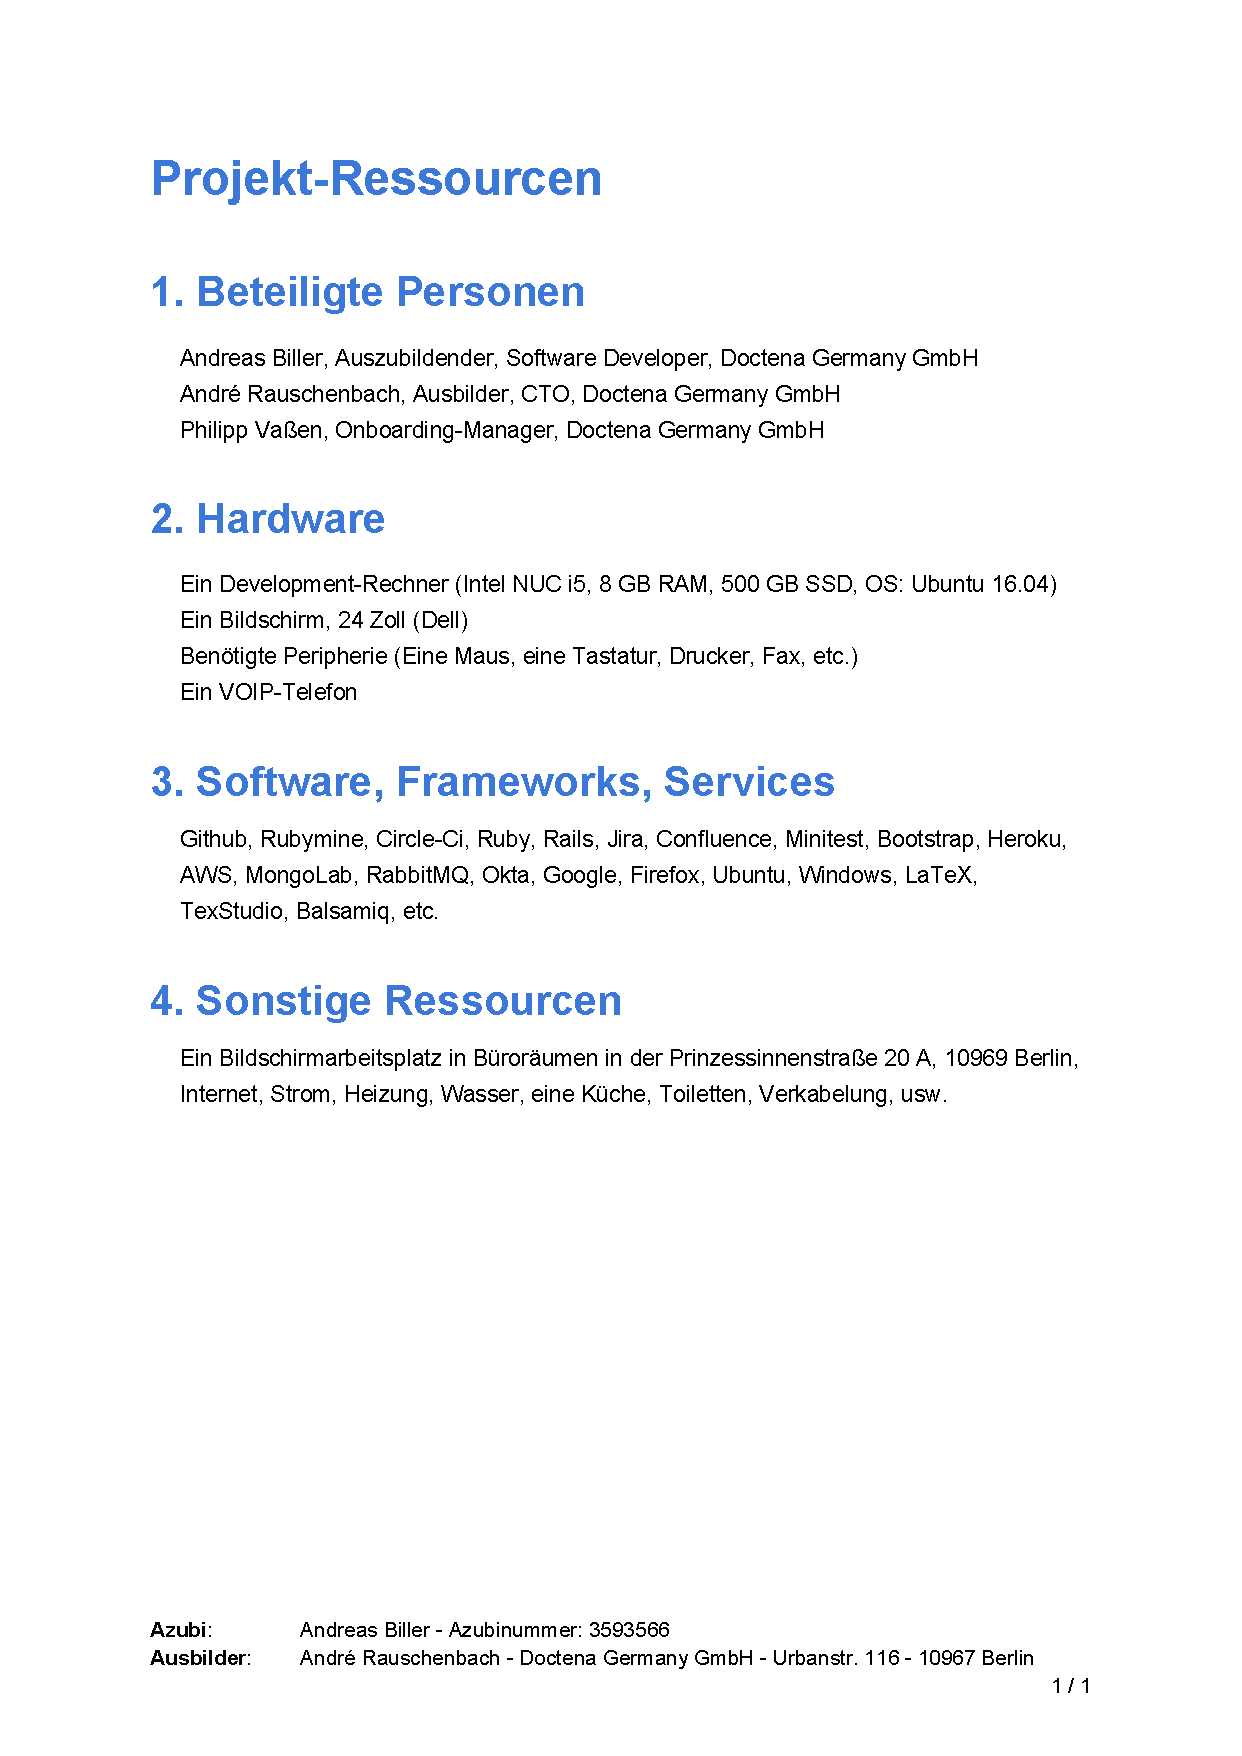
\includepdf[scale=0.8,clip,trim=0cm 0cm 0cm 0cm,offset=0 -2cm,pages={1},pagecommand={\section{Anhang}\subsection{Projekt-Ressourcen}\label{app:Ressourcen}}]{Projektressourcen.pdf}
\clearpage

% \subsection{Lastenheft}
\label{app:Lastenheft}
Es folgt unser Lastenheft mit Fokus auf den Anforderungen:

Die Umsetzung muss folgende Anforderungen erfüllen: 
\begin{enumerate}[itemsep=0em,partopsep=0em,parsep=0em,topsep=0em]
\item DMZ
	\begin{enumerate}
	\item Die DMZ soll aus zwei virtuellen, zu Routern konfigurierten Linux-Distributionen bestehen, welch die Netze INSIDE, OUTSIDE und das DMZ-Netz miteinander verbinden. 
	\item Die Router sollen entsprechend des Netzplanes eingerichtet und konfiguriert werden.
	\item Die DMZ soll Zugriffe auf den Webserver erlauben, aber Zugriffe auf das INSIDE-Netz verhindern. Hierzu soll auf dem Outside-Router NAT, Portforwarding und eine Firewall laufen.
    \item Die Router sollen nur vom Client-Rechner her fernadministrierbar sein.
	\end{enumerate}
\item Client-Rechner
\begin{enumerate}
    \item Der Client-Rechner im INSIDE-Netz nutzt das Betriebssystem Windows.
    \item Der Webserver soll eine Webseite mit dem aktuellen Stand der Gruppe anzeigen.    
\end{enumerate}
\item Webserver
\begin{enumerate}
    \item Der Webserver nutzt das Betriebssystem Windows. Er wird über das Tool Mini-Webserver vom Auftraggeber bereitgestellt.
    \item Der Webserver im DMZ-Netz muss vom OUTSIDE-Netz über Port 80 erreichbar sein. Hierzu soll auf dem Outside-Router NAT und Port-Forwarding eingerichtet werden.
    \item Der Webserver soll eine Webseite mit dem aktuellen Stand der Gruppe anzeigen.    
\end{enumerate}
\item Firewall
\begin{enumerate}
    \item Die Firewall soll den Webserver in der DMZ über Port 80 erreichbar sein lassen.
    \item Die Firewall soll SSH nur vom Admin-PC zulassen.
    \item Die Firewall soll ICMP zulassen.
    \item Die Firewall soll DNS zulassen.
    \item Die Firewall soll RDP zulassen.
    \item Die Firewall soll per Script an- und ausschaltbar sein. Hierzu muss an diversen Stellen per Script die Linux-Systemkonfiguration verändert werden
\end{enumerate}
\item Sonstige Anforderungen
	\begin{enumerate}
	\item Das Projekt soll unter Berücksichtigung der von der IHK ausgegebenen Richtlinien für eine Projektdokumentation dokumentiert werden.
    \item Es soll ein logischer Netzplan in Papierform erstellt und der Dokumentation angefügt werden.
	\item Pro Person soll ein ausführliches Kompetenzportfolio erstellt werden, welches einen kritischen Überblick über unsere individuellen Kompetenzstände vor, während und nach dem Projekt liefert. Diese sollen der Dokumentation angehängt werden.
	\item Die Funktionalität der Firewall soll getestet und die Ergebnisse in zwei Testprotokollen festgehalten werden. Diese sind der Dokumentation anzuhängen.
	\end{enumerate}
\end{enumerate}


% \subsection{Pflichtenheft}
\label{app:Pflichtenheft}

Unser aus den Anforderungen des Lastenheftes erstelltes Pflichtenheft:

\begin{enumerate}[itemsep=0em,partopsep=0em,parsep=0em,topsep=0em]
\item Musskriterien % Wikipedia: für das Produkt unabdingbare Leistungen, die in jedem Fall erfüllt werden müssen
    \begin{enumerate}
    \item Das DMZ-Netz erhält die Netzmaske 172.16.9.0/24
    \item Das intere Netz erhält die Netzmaske 10.0.9.0/24
    \item Die öffentliche Schnittstelle des Outside-Router erhält die IP 192.168.200.109
    \item Der Outside-Router erhält als Standard-Gateway die IP 192.168.200.1
    \item Der Outside-Router erhält eine statische Route für das interne und DMZ-Netz
    \item Der Inside-Router erhält als Standard-Gateway das Interface des Outside-Routers, welches in die DMZ zeigt
    \item Der Webserver ist über die öffentliche IP des Outside-Routers über HTTP/S von außen erreichbar
    \item Der Webserver ist über die lokale IP 172.16.9.3 über HTTP/S aus dem internen Netzwerk erreichbar
    \item Die Router und Windows-Clients bekommen als DNS-Server die IPs 192.168.95.40 und 192.168.95.41
    \item Die Router und Windows-Clients bekommen als NTP-Server die IP 192.168.200.1
    \item Die Firewall verhindert unrechtmäßigen Datentransfer zwischen den Netzen und auf den Routern
    \item Der Admin-PC mit der IP 10.0.9.2 ist berechtigt mittels SSH auf die Router zuzugreifen	
    \end{enumerate}
\item Kannkriterien
    \begin{enumerate}
    \item Die Firewall lässt sich mit den Optionen "start" und "stop" an- bzw.\ ausschalten
    \item Die Firewall-Scripts der Router befinden sich im Verzeichnis /root/bin
    \item Die Veränderung der Firewall-Konfiguration befindet sich jeweils im Verzeichnis /var/log/firewall
    \item Der Admin-PC mit der IP 10.0.9.2 ist berechtigt mittels RDP auf den Webserver zuzugreifen
    \end{enumerate}
\end{enumerate}
	
% \clearpage

% \subsection{Netzpläne}
% \label{app:Netzplan}
% Der Netzplan unserer \ac{DMZ} in der Projektumgebung im Labor 3.1.01:
% \begin{figure}[htb]
% \centering
% \includegraphicsKeepAspectRatio{PLZNetzplanProjektumgebung.png}{0.8}
% \caption{Netzplan der \ac{DMZ} in Raum 3.1.01 (Arbeitsgruppe 9)}
% \end{figure}

% Der Netzplan unserer \ac{DMZ} in der virtualisierten Testumgebung:
% \begin{figure}[htb]
%     \centering
%     \includegraphicsKeepAspectRatio{PLZNetzplanTestumgebung.png}{0.8}
%     \caption{Netzplan der erweiterten \ac{DMZ} in unserer virtuellen Testumgebung}
% \end{figure}
% \clearpage

% 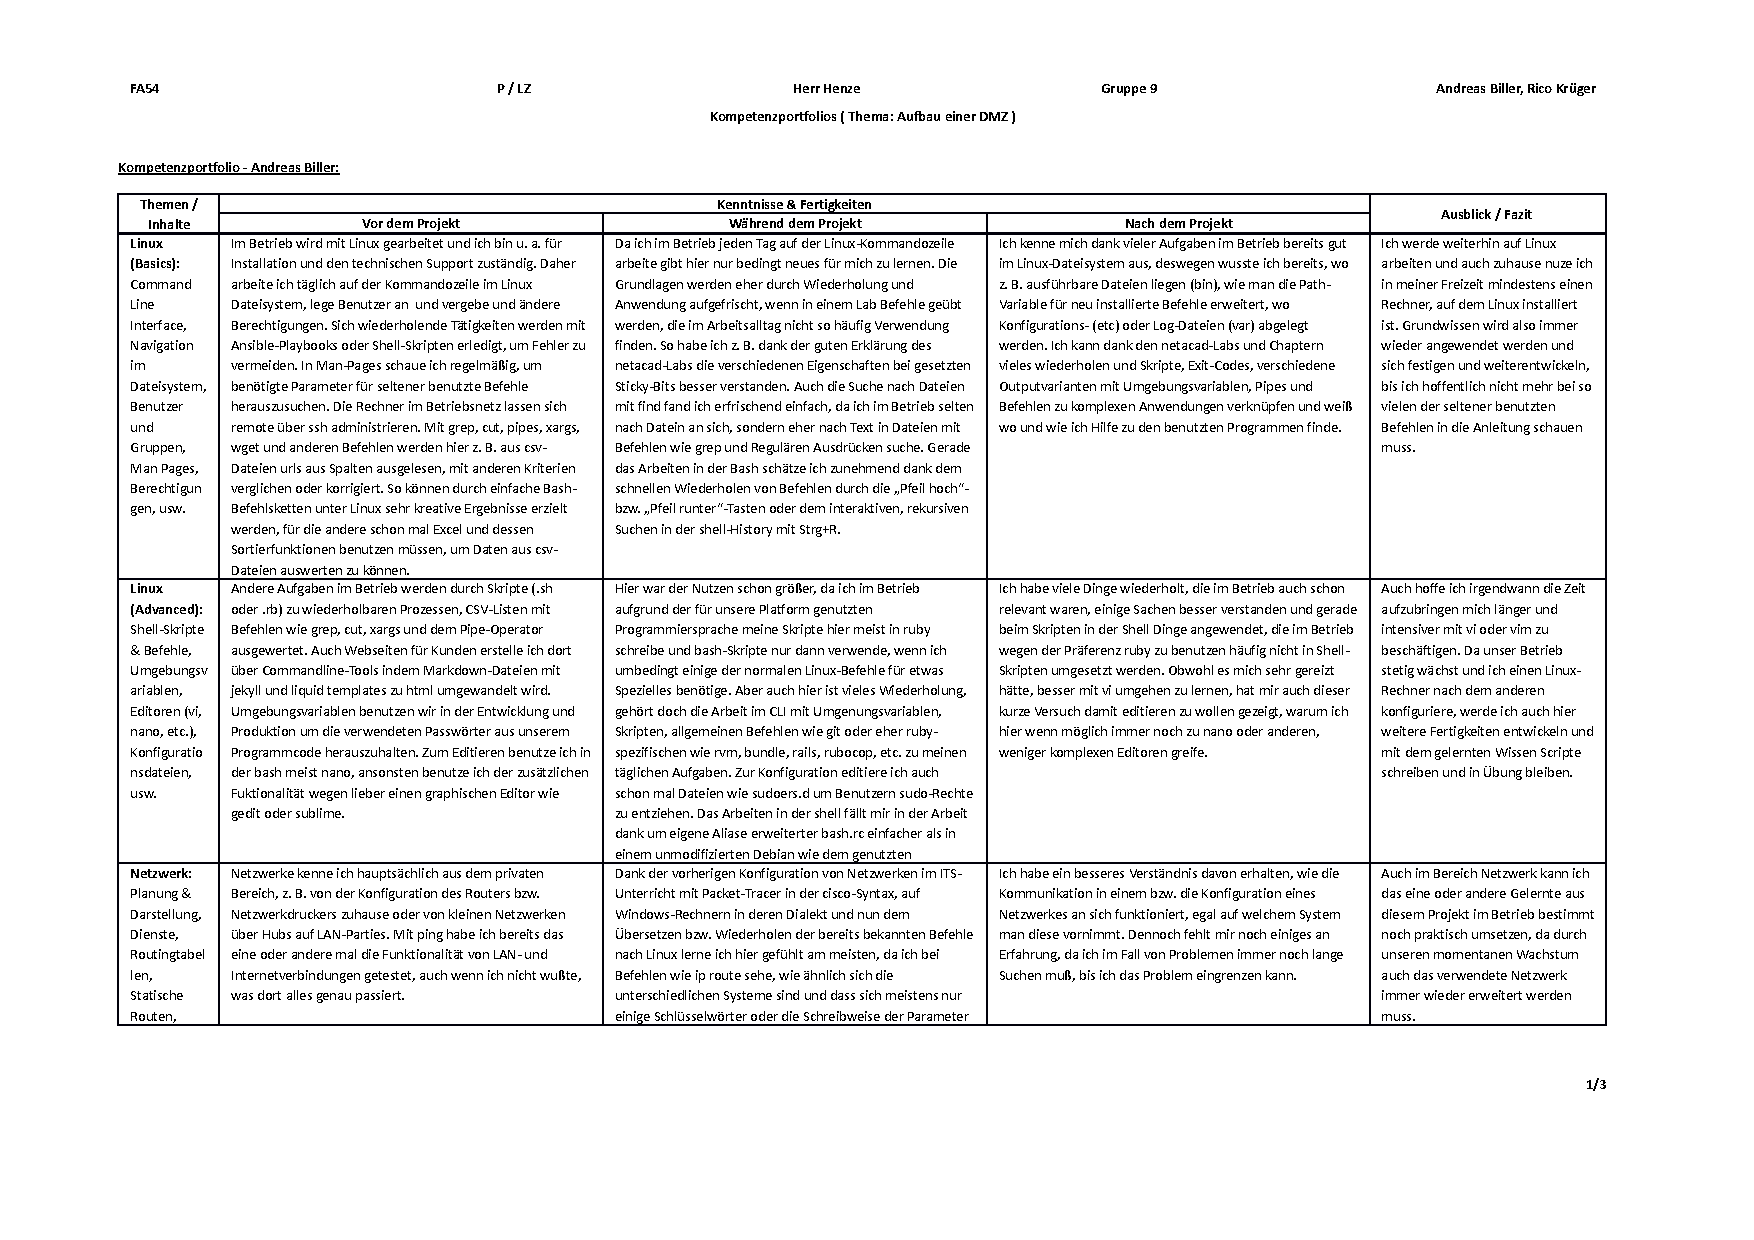
\includepdf[scale=0.925,clip,trim=0cm 0cm 0cm 0cm,offset=0.7cm -1cm,landscape=true,pages={1},pagecommand={\subsection{Kompetenzportfolios}\label{app:Kompetenz}}]{Kompetenzportfolios.pdf}
% \includepdf[scale=0.95,clip,trim=0cm 0cm 0cm 0cm,offset=0.5cm -0.4cm,landscape=true,pages={2-3},pagecommand={}]{Kompetenzportfolios.pdf}
% \clearpage

% \section{Testdokumentation}
% \label{app:Test}

% \begin{table}[!ht]
    \tabelleAnhang{Systeminformation}{tab:Systeminformation}{Systeminformation.tex}
    \caption{Hardwaredetails des Testsystems}
    \label{tab:tabletestsystem}
\end{table}

\subsection{Aufbau der Testumgebung}
\label{app:testaufbau}
Die zur Umsetzung dieses Kapitels benötigten Informationen entstammen unter anderem den hilfreichen Artikeln folgender Webseiten: \cite{networkdriverhacking}

\subsubsection{Implementierung der Virtuellen Maschinen}
Im Server-Manager fügen wir über \textit{Verwalten > Rollen und Features hinzufügen} den Hyper-V-Manager hinzu indem wir dem Assistenten folgen. Dieser gestattet es virtuelle Maschinen und Netzwerke zu installieren.
Als nächstes wird eine neue virtuelle Linux (Debian 7.1)  Maschine (Generation 1) aus einem Image erstellt. Dies geschieht mit Hilfe eines Assistenten. Sie bekommt einen virtuellen Prozessor und 1 \ac{GB} Arbeitsspeicher. Des weiteren wird bei der Installation eine 5 \ac{GB} große Festplatte für die Maschine erstellt und ihr zugewiesen. Als virtuellen Switch weisen wir ihr vorläufig den Netzwerkadapter des Hosts zu. Somit besitzt unsere Linux-\ac{VM} Internet. Um sie zu installieren, startet man nun die Maschine und verbindet sich zu ihr. Danach folgt man wie gewohnt den Installationsschritten wie bei einer physischen Maschine. Danach installieren wir den \ac{NTP}-Service. Ist die Grundkonfiguration fertig, wird die Maschine ausgeschaltet.
Die Installation der Windows 7 \ac{VM} erfolgt analog zu die der Linux \ac{VM}. Wir vergeben jedoch 4 \ac{GB} \ac{RAM} und erstellen eine mindestens 30 \ac{GB} große virtuelle Festplatte. Nach der Installation wird die Firewall wie in \nameref{sec:Implementierungsphase} eingerichtet. Zusätzlich werden noch nützliche Software wie putty oder winscp heruntergeladen.
Nach der Grundkonfiguration der beiden \ac{VM}s können diese nun dupliziert werden. Dazu muss man die virtuelle Maschine erst exportieren, um sie danach wieder zu importieren. Beim Import sollte man darauf achten, dass man \textit{eine neue eindeutige \ac{ID} } erstellt. Nachdem starten der importierten Maschine wird als erstes der Hostname geändert, um sie von der Originalen zu unterscheiden und um \ac{DNS}-Konflikte zu vermeiden.

\subsubsection{Implementierung des virtuellen Netzwerkes}
Virtuelle Netzwerke werden über das Hinzufügen virtueller Switche an den Netzwerkadaptern der virtuellen Maschine erstellt. Auf diesen lassen sich auch \ac{VLAN}s einrichten.
Die Installation eines solchen Switch wird ebenfalls vom Hyper-V-Manager mit einem Assistenten bereitgestellt. Für Testzwecke werden 2 \textit{private} Switche erstellt, da diese die direkte Kommunikation mit dem Host unterbinden und somit nicht die Router umgangen werden. Diese erhalten den Namen \ac{DMZ}- \bzw \ac{LAN}-Switch. Ein \textit{öffentlicher} Switch ist bereits vorhanden. Mit diesem ist der physische Netzwerkadapter des Hosts verbunden. Diese werden dann den \ac{VM}s entsprechend des \nameref{app:Netzplan}s zugeordnet. Für die Linux-\ac{VM}s, die als Router fungieren, muss \evtl noch ein zweiter Netzwerkadapter hinzugefügt werden. Nun können die Router und Clients (\text{Siehe Bild und Implementierung}) konfiguriert werden.

\subsubsection{Implementierung des \ac{DNS}-Servers}
Der \ac{DNS}-Server wird ebenfalls über den Server-Manager (unter \textit{Rollen und Features hinzufügen}) installiert. Diesen kann man nun über den \ac{DNS}-Manager verwalten. Es genügt eine \textit{Forward-Lookup}-Zone zu erstellen. Als Zonennamen wählen wir \textit{fritz.box} da bereits das Standard-Gateway darauf verweist. Dies ist die Domäne bzw. das \ac{DNS}-Suffix. Dieses Suffix wird auf den Windows-\ac{VM}s in den \ac{IP}v4-Einstellungen des Netzwerkadapters nachgetragen. Auf den Linux-\ac{VM}s tragen wir dies zusätzlich in die \verb+/etc/resolv.conf+ vor unserem \ac{DNS}-Server ein. \textbf{siehe resolv.conf oder selber schreiben]
Über den \ac{DNS}-Manager werden im Anschluss noch in der Zone \textit{fritz.box} unsere \ac{VM}s (A-Record) mit Namen und \ac{IP}-Adressen eingetragen. \textbf Siehe \ac{DNS}Manager.png}.

\subsubsection{Testen der Firewall}
Nachdem das Firewall-Script auf die Router kopiert und die \ac{DNS}-Server angepasst wurden, kann mit den Tests begonnen und die Firewall ggf.\ angepasst werden. Dazu speichern wir den Verlauf der erstellten Regeln als Log-Ausgabe in \verb+/var/log/firewall/firewallConfig+ ab. Die Ergebnisse unserer Tests finden sich als Übersicht in den folgenden Tabellen der Testprotokolle:


% Testprotokolle
\subsubsection{Testprotokolle}
\label{app:Testprotokolle}
% Description
\clearpage

% tables created with: http://www.tablesgenerator.com/latex_tables
% Please add the following required packages to your document preamble:
% \usepackage{graphicx}
% \usepackage[table,xcdraw]{xcolor}
% If you use beamer only pass "xcolor=table" option, i.e. \documentclass[xcolor=table]{beamer}
\begin{table}[!ht]
    \resizebox{\textwidth}{!}{%
        \begin{tabular}{llllll}
            \rowcolor[HTML]{009BA7} 
            \textbf{Service} & \textbf{Command} & \textbf{Source-IP} & \textbf{Destination-IP} & \textbf{Soll} & \textbf{Ist} \\
            ICMP & ping & 10.0.9.2 & 10.0.9.1 & ja & ja \\
            \rowcolor[HTML]{EFEFEF} 
            ICMP & ping & 10.0.9.3 & 10.0.9.1 & ja & ja \\
            ICMP & ping & 10.0.9.2 & 172.16.9.1 & ja & ja \\
            \rowcolor[HTML]{EFEFEF} 
            ICMP & ping & 10.0.9.3 & 172.16.9.1 & ja & ja \\
            ICMP & ping & 172.16.9.3 & 172.16.9.1 & ja & ja \\
            \rowcolor[HTML]{EFEFEF} 
            ICMP & ping & 172.16.9.3 & 172.16.9.2 & ja & ja \\
            ICMP & ping & 10.0.9.3 & 192.168.200.10 & ja & ja \\
            \rowcolor[HTML]{EFEFEF} 
            ICMP & ping & 192.168.200.10 & 10.0.9.3 & ja & ja \\
            ICMP & ping & 192.168.200.10 & 172.16.9.3 & ja & ja \\
            \rowcolor[HTML]{EFEFEF} 
            ICMP & ping & 192.168.200.10 & 192.168.200.109 & ja & ja \\
            ICMP & ping & 10.0.9.3 & 8.8.8.8 & ja & ja \\
            \rowcolor[HTML]{EFEFEF} 
            HTTP & http://172.16.9.3 & 192.168.200.10 & 192.168.200.109 & ja & ja \\
            HTTP & http://172.16.9.3 & 192.168.200.10 & 172.16.9.3 & ja & ja \\
            \rowcolor[HTML]{EFEFEF} 
            HTTP & http://172.16.9.3 & 10.0.9.3 & 192.168.200.109 & ja & ja \\
            HTTP & http://172.16.9.3 & 10.0.9.3 & 172.16.9.3 & ja & ja \\
            \rowcolor[HTML]{EFEFEF} 
            NTP & w32tm /stripchart /computer:192.168.200.1 & 10.0.9.2 & 192.168.200.1 & ja & ja \\
            NTP & w32tm /stripchart /computer:192.168.200.1 & 172.16.9.3 & 192.168.200.1 & ja & ja \\
            \rowcolor[HTML]{EFEFEF} 
            NTP & ntpq -p & 192.168.200.109 & 192.168.200.1 & ja & ja \\
            RDP & mstsc.exe & 10.0.9.2 & 172.16.9.3 & ja & ja \\
            \rowcolor[HTML]{EFEFEF} 
            RDP & mstsc.exe & 10.0.9.3 & 172.16.9.3 & ja & ja \\
            SSH & putty & 10.0.9.2 & 10.0.9.1 & ja & ja \\
            \rowcolor[HTML]{EFEFEF} 
            SSH & putty & 10.0.9.2 & 172.16.9.1 & ja & ja \\
            SSH & putty & 10.0.9.3 & 10.0.9.1 & ja & ja \\
            \rowcolor[HTML]{EFEFEF} 
            SSH & putty & 10.0.9.3 & 172.16.9.1 & ja & ja \\
            SSH & putty & 172.16.9.3 & 172.16.9.1 & ja & ja \\
            \rowcolor[HTML]{EFEFEF} 
            SSH & putty & 172.16.9.3 & 172.16.9.2 & ja & ja \\
            DNS & nslookup 172.16.9.1 & 10.0.9.3 & 192.168.200.10 & ja & ja \\
            \rowcolor[HTML]{EFEFEF} 
            DNS & nslookup Inside-Router & 172.16.9.3 & 192.168.200.10 & ja & ja \\
            DNS & nslookup 10.0.9.1 & 172.16.9.2 & 192.168.200.10 & ja & ja \\
            \rowcolor[HTML]{EFEFEF} 
            DNS & nslookup Client-PC & 192.168.200.109 & 192.168.200.10 & ja & ja
        \end{tabular}%
    }
    \caption{Aus - Aus}
    \label{tab:ausaus}
\end{table}

% Please add the following required packages to your document preamble:
% \usepackage{graphicx}
% \usepackage[table,xcdraw]{xcolor}
% If you use beamer only pass "xcolor=table" option, i.e. \documentclass[xcolor=table]{beamer}
\begin{table}[!ht]
    \resizebox{\textwidth}{!}{%
        \begin{tabular}{llllll}
            \rowcolor[HTML]{009BA7} 
            \textbf{Service} & \textbf{Command} & \textbf{Source-IP} & \textbf{Destination-IP} & \textbf{Soll} & \textbf{Ist} \\
            ICMP & ping & 10.0.9.2 & 10.0.9.1 & ja & ja \\
            \rowcolor[HTML]{EFEFEF} 
            ICMP & ping & 10.0.9.3 & 10.0.9.1 & nein & nein \\
            ICMP & ping & 10.0.9.2 & 172.16.9.1 & ja & ja \\
            \rowcolor[HTML]{EFEFEF} 
            ICMP & ping & 10.0.9.3 & 172.16.9.1 & nein & nein \\
            ICMP & ping & 172.16.9.3 & 172.16.9.1 & ja & ja \\
            \rowcolor[HTML]{EFEFEF} 
            ICMP & ping & 172.16.9.3 & 172.16.9.2 & nein & nein \\
            ICMP & ping & 10.0.9.3 & 192.168.200.10 & ja & ja \\
            \rowcolor[HTML]{EFEFEF} 
            ICMP & ping & 192.168.200.10 & 10.0.9.3 & nein & nein \\
            ICMP & ping & 192.168.200.10 & 172.16.9.3 & ja & ja \\
            \rowcolor[HTML]{EFEFEF} 
            ICMP & ping & 192.168.200.10 & 192.168.200.109 & ja & ja \\
            ICMP & ping & 10.0.9.3 & 8.8.8.8 & ja & ja \\
            \rowcolor[HTML]{EFEFEF} 
            HTTP & http://172.16.9.3 & 192.168.200.10 & 192.168.200.109 & ja & ja \\
            HTTP & http://172.16.9.3 & 192.168.200.10 & 172.16.9.3 & ja & ja \\
            \rowcolor[HTML]{EFEFEF} 
            HTTP & http://172.16.9.3 & 10.0.9.3 & 192.168.200.109 & nein & nein \\
            HTTP & http://172.16.9.3 & 10.0.9.3 & 172.16.9.3 & ja & ja \\
            \rowcolor[HTML]{EFEFEF} 
            NTP & w32tm /stripchart /computer:192.168.200.1 & 10.0.9.2 & 192.168.200.1 & ja & ja \\
            NTP & w32tm /stripchart /computer:192.168.200.1 & 172.16.9.3 & 192.168.200.1 & ja & ja \\
            \rowcolor[HTML]{EFEFEF} 
            NTP & ntpq -p & 192.168.200.109 & 192.168.200.1 & ja & ja \\
            RDP & mstsc.exe & 10.0.9.2 & 172.16.9.3 & ja & ja \\
            \rowcolor[HTML]{EFEFEF} 
            RDP & mstsc.exe & 10.0.9.3 & 172.16.9.3 & nein & nein \\
            SSH & putty & 10.0.9.2 & 10.0.9.1 & ja & ja \\
            \rowcolor[HTML]{EFEFEF} 
            SSH & putty & 10.0.9.2 & 172.16.9.1 & ja & ja \\
            SSH & putty & 10.0.9.3 & 10.0.9.1 & nein & nein \\
            \rowcolor[HTML]{EFEFEF} 
            SSH & putty & 10.0.9.3 & 172.16.9.1 & ja & ja \\
            SSH & putty & 172.16.9.3 & 172.16.9.1 & ja & ja \\
            \rowcolor[HTML]{EFEFEF} 
            SSH & putty & 172.16.9.3 & 172.16.9.2 & nein & nein \\
            DNS & nslookup 172.16.9.1 & 10.0.9.3 & 192.168.200.10 & ja & ja \\
            \rowcolor[HTML]{EFEFEF} 
            DNS & nslookup Inside-Router & 172.16.9.3 & 192.168.200.10 & ja & ja \\
            DNS & nslookup 10.0.9.1 & 172.16.9.2 & 192.168.200.10 & ja & ja \\
            \rowcolor[HTML]{EFEFEF} 
            DNS & nslookup Client-PC & 192.168.200.109 & 192.168.200.10 & ja & ja
        \end{tabular}%
    }
    \caption{Aus - An}
    \label{tab:ausan}
\end{table}

% Please add the following required packages to your document preamble:
% \usepackage{graphicx}
% \usepackage[table,xcdraw]{xcolor}
% If you use beamer only pass "xcolor=table" option, i.e. \documentclass[xcolor=table]{beamer}
\begin{table}[!ht]
    \resizebox{\textwidth}{!}{%
        \begin{tabular}{llllll}
            \rowcolor[HTML]{009BA7} 
            \textbf{Service} & \textbf{Command} & \textbf{Source-IP} & \textbf{Destination-IP} & \textbf{Soll} & \textbf{Ist} \\
            ICMP & ping & 10.0.9.2 & 10.0.9.1 & ja & ja \\
            \rowcolor[HTML]{EFEFEF} 
            ICMP & ping & 10.0.9.3 & 10.0.9.1 & ja & ja \\
            ICMP & ping & 10.0.9.2 & 172.16.9.1 & ja & ja \\
            \rowcolor[HTML]{EFEFEF} 
            ICMP & ping & 10.0.9.3 & 172.16.9.1 & nein & nein \\
            ICMP & ping & 172.16.9.3 & 172.16.9.1 & nein & nein \\
            \rowcolor[HTML]{EFEFEF} 
            ICMP & ping & 172.16.9.3 & 172.16.9.2 & ja & ja \\
            ICMP & ping & 10.0.9.3 & 192.168.200.10 & ja & ja \\
            \rowcolor[HTML]{EFEFEF} 
            ICMP & ping & 192.168.200.10 & 10.0.9.3 & nein & nein \\
            ICMP & ping & 192.168.200.10 & 172.16.9.3 & nein & nein \\
            \rowcolor[HTML]{EFEFEF} 
            ICMP & ping & 192.168.200.10 & 192.168.200.109 & nein & nein \\
            ICMP & ping & 10.0.9.3 & 8.8.8.8 & ja & ja \\
            \rowcolor[HTML]{EFEFEF} 
            HTTP & http://172.16.9.3 & 192.168.200.10 & 192.168.200.109 & ja & ja \\
            HTTP & http://172.16.9.3 & 192.168.200.10 & 172.16.9.3 & ja & ja \\
            \rowcolor[HTML]{EFEFEF} 
            HTTP & http://172.16.9.3 & 10.0.9.3 & 192.168.200.109 & nein & nein \\
            HTTP & http://172.16.9.3 & 10.0.9.3 & 172.16.9.3 & ja & ja \\
            \rowcolor[HTML]{EFEFEF} 
            NTP & w32tm /stripchart /computer:192.168.200.1 & 10.0.9.2 & 192.168.200.1 & ja & ja \\
            NTP & w32tm /stripchart /computer:192.168.200.1 & 172.16.9.3 & 192.168.200.1 & ja & ja \\
            \rowcolor[HTML]{EFEFEF} 
            NTP & ntpq -p & 192.168.200.109 & 192.168.200.1 & ja & ja \\
            RDP & mstsc.exe & 10.0.9.2 & 172.16.9.3 & ja & ja \\
            \rowcolor[HTML]{EFEFEF} 
            RDP & mstsc.exe & 10.0.9.3 & 172.16.9.3 & nein & nein \\
            SSH & putty & 10.0.9.2 & 10.0.9.1 & ja & ja \\
            \rowcolor[HTML]{EFEFEF} 
            SSH & putty & 10.0.9.2 & 172.16.9.1 & ja & ja \\
            SSH & putty & 10.0.9.3 & 10.0.9.1 & ja & ja \\
            \rowcolor[HTML]{EFEFEF} 
            SSH & putty & 10.0.9.3 & 172.16.9.1 & ja & ja \\
            SSH & putty & 172.16.9.3 & 172.16.9.1 & nein & nein \\
            \rowcolor[HTML]{EFEFEF} 
            SSH & putty & 172.16.9.3 & 172.16.9.2 & ja & ja \\
            DNS & nslookup 172.16.9.1 & 10.0.9.3 & 192.168.200.10 & ja & ja \\
            \rowcolor[HTML]{EFEFEF} 
            DNS & nslookup Inside-Router & 172.16.9.3 & 192.168.200.10 & ja & ja \\
            DNS & nslookup 10.0.9.1 & 172.16.9.2 & 192.168.200.10 & ja & ja \\
            \rowcolor[HTML]{EFEFEF} 
            DNS & nslookup Client-PC & 192.168.200.109 & 192.168.200.10 & ja & ja
        \end{tabular}%
    }
    \caption{An - Aus}
    \label{tab:anaus}
\end{table}

% Please add the following required packages to your document preamble:
% \usepackage{graphicx}
% \usepackage[table,xcdraw]{xcolor}
% If you use beamer only pass "xcolor=table" option, i.e. \documentclass[xcolor=table]{beamer}
\begin{table}[!ht]
    \resizebox{\textwidth}{!}{%
        \begin{tabular}{llllll}
            \rowcolor[HTML]{009BA7} 
            \textbf{Service} & \textbf{Command} & \textbf{Source-IP} & \textbf{Destination-IP} & \textbf{Soll} & \textbf{Ist} \\
            ICMP & ping & 10.0.9.2 & 10.0.9.1 & ja & ja \\
            \rowcolor[HTML]{EFEFEF} 
            ICMP & ping & 10.0.9.3 & 10.0.9.1 & ja & ja \\
            ICMP & ping & 10.0.9.2 & 172.16.9.1 & ja & ja \\
            \rowcolor[HTML]{EFEFEF} 
            ICMP & ping & 10.0.9.3 & 172.16.9.1 & nein & nein \\
            ICMP & ping & 172.16.9.3 & 172.16.9.1 & nein & nein \\
            \rowcolor[HTML]{EFEFEF} 
            ICMP & ping & 172.16.9.3 & 172.16.9.2 & ja & ja \\
            ICMP & ping & 10.0.9.3 & 192.168.200.10 & ja & ja \\
            \rowcolor[HTML]{EFEFEF} 
            ICMP & ping & 192.168.200.10 & 10.0.9.3 & nein & nein \\
            ICMP & ping & 192.168.200.10 & 172.16.9.3 & nein & nein \\
            \rowcolor[HTML]{EFEFEF} 
            ICMP & ping & 192.168.200.10 & 192.168.200.109 & nein & nein \\
            ICMP & ping & 10.0.9.3 & 8.8.8.8 & ja & ja \\
            \rowcolor[HTML]{EFEFEF} 
            HTTP & http://172.16.9.3 & 192.168.200.10 & 192.168.200.109 & ja & ja \\
            HTTP & http://172.16.9.3 & 192.168.200.10 & 172.16.9.3 & ja & ja \\
            \rowcolor[HTML]{EFEFEF} 
            HTTP & http://172.16.9.3 & 10.0.9.3 & 192.168.200.109 & nein & nein \\
            HTTP & http://172.16.9.3 & 10.0.9.3 & 172.16.9.3 & ja & ja \\
            \rowcolor[HTML]{EFEFEF} 
            NTP & w32tm /stripchart /computer:192.168.200.1 & 10.0.9.2 & 192.168.200.1 & ja & ja \\
            NTP & w32tm /stripchart /computer:192.168.200.1 & 172.16.9.3 & 192.168.200.1 & ja & ja \\
            \rowcolor[HTML]{EFEFEF} 
            NTP & ntpq -p & 192.168.200.109 & 192.168.200.1 & ja & ja \\
            RDP & mstsc.exe & 10.0.9.2 & 172.16.9.3 & ja & ja \\
            \rowcolor[HTML]{EFEFEF} 
            RDP & mstsc.exe & 10.0.9.3 & 172.16.9.3 & nein & nein \\
            SSH & putty & 10.0.9.2 & 10.0.9.1 & ja & ja \\
            \rowcolor[HTML]{EFEFEF} 
            SSH & putty & 10.0.9.2 & 172.16.9.1 & ja & ja \\
            SSH & putty & 10.0.9.3 & 10.0.9.1 & ja & ja \\
            \rowcolor[HTML]{EFEFEF} 
            SSH & putty & 10.0.9.3 & 172.16.9.1 & ja & ja \\
            SSH & putty & 172.16.9.3 & 172.16.9.1 & nein & nein \\
            \rowcolor[HTML]{EFEFEF} 
            SSH & putty & 172.16.9.3 & 172.16.9.2 & ja & ja \\
            DNS & nslookup 172.16.9.1 & 10.0.9.3 & 192.168.200.10 & ja & ja \\
            \rowcolor[HTML]{EFEFEF} 
            DNS & nslookup Inside-Router & 172.16.9.3 & 192.168.200.10 & ja & ja \\
            DNS & nslookup 10.0.9.1 & 172.16.9.2 & 192.168.200.10 & ja & ja \\
            \rowcolor[HTML]{EFEFEF} 
            DNS & nslookup Client-PC & 192.168.200.109 & 192.168.200.10 & ja & ja
        \end{tabular}%
    }
    \caption{An - An}
    \label{tab:anan}
\end{table}
\clearpage

\subsection{Firewall-Skripte}
\label{app:Firewall}

\subsubsection{firewall.sh (auf dem Outside-Router)}
\label{app:Firewall-Outside}
\lstinputlisting[language=sh]{Listings/outside/firewall.sh}

\subsubsection{firewall.sh (auf dem Inside-Router)}
\label{app:Firewall-Inside}
\lstinputlisting[language=sh]{Listings/inside/firewall.sh}




\end{document}
